\chapter{Background}
\label{ch:background}

\graphicspath{{mainmatter/background/figures/}}

\label{sec:background:preface}

In \cref{ch:introduction}, we defined a common set of (artificial) intelligence-based cloud services that we label \glsplx{iws}. Specifically, we scope the primary body of this study's work on \glsplx{cvs} (e.g., Google Cloud Vision \citep{GoogleCloud:Home}, AWS Rekognition \citep{AWS:Home}, Azure Computer Vision \citep{Azure:Home}, Watson Visual Recognition \citep{IBM:Home} etc.). We claim developers have a distinctly deterministic mindset ($2+2$ \textit{always}  equals 4) whereas an \gls{iws}'s `intelligence' component (a black box) may return probabilistic results ($2+2$ \textit{might} equal 4 \textit{with a confidence of} 95\%). Thus, there is a mindset mismatch between probabilistic results (from the \gls{api} provider) and results interpreted with certainty (from the \gls{api} consumer).

What affect does this mindset mismatch have on the developer's approach towards building probabilistic software? What can we learn from common software engineering practices (e.g., \citep{Pressman:2005vf,Sommerville:2011uc}) that apply to resolve this mismatch and thereby improve quality, such as \gls{vv}? Chiefly, we anchor this question around three lenses of software engineering: creating an \gls{iws}, using an \gls{iws}, and the nature of \glspl{iws} themselves.

Our chief concern lies with interaction and integration between \gls{iws} providers and consumers, the nature of applications built using an \gls{iws}, and the impact this has on software quality. We triangulate this around three pillars, which we diagrammatically represent in \cref{fig:background:preface:iws-mindset-clash-pillars}.
 
\begin{enumerate}[label=\textbf{(\arabic*})]
\item \textbf{The development of the \gls{iws}.} We investigate the internal quality attributes of creating an \gls{iws} from the \gls{iws} \textit{provider's} perspective. That is, we ask if existing verification techniques are sufficient enough to ensure that the \gls{iws} being developed actually satisfies the \gls{iws} consumer's needs and if the internal perspective of creating the system with a non-deterministic mindset clashes with the outside perspective (i.e., pillar 2).
\item \textbf{The usage of the \gls{iws}.} We investigate the external quality attributes of using an \gls{iws} from the \gls{iws} \textit{consumer's} perspective. That is, we ask if existing validation techniques are sufficient enough to ensure that the end-users can actually use an \gls{iws} to build their software in the ways they expect the \gls{iws} to work.
\item \textbf{The nature of an \gls{iws}.} We investigate what standard software engineering practices apply when developing non-deterministic systems. That is, we tackle what best practices exist when developing systems that are inherently stochastic and probabilistic, i.e., the `black box' intelligence itself.
\end{enumerate}

\begin{figure}[hbt]
  \centering
  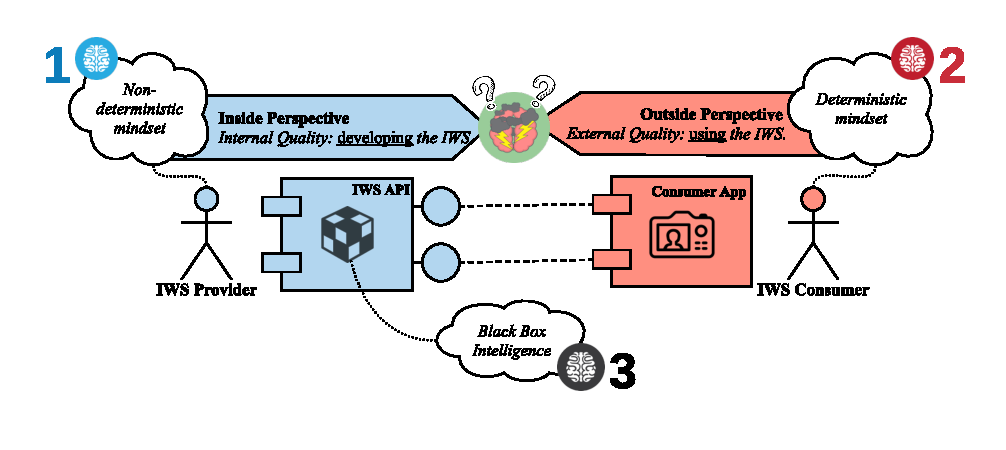
\includegraphics[width=\linewidth]{iws-mindset-clash-pillars}
  \caption[Mindset clashes within the development, use and nature of a IWS]{The three pillars by which we anchor the background: (1) developing an \gls{iws} with a non-deterministic mindset by the \gls{iws} provider; (2) the use of a \gls{iws} with a deterministic mindset by the \gls{iws} consumer; (3) the nature of a \gls{iws} itself.}
  \label{fig:background:preface:iws-mindset-clash-pillars}
\end{figure}

Does a clash of deterministic consumer mindsets who use a \gls{iws} and the non-deterministic provider mindsets who develop them exist? And what impact does this have on the inside and outside perspective? Throughout this chapter, we will review these three core pillars due to such  mindset mismatch from the anchoring perspective of software quality, particularly around \gls{vv} and related quality attributes, probabilistic and nondeterministic software and the nature of \glspl{api}. 

\section{Software Quality}
\label{sec:background:software-quality}

\epigraph{Quality... you know what it is, yet you don't know what it is.}{Robert Pirsig, 1974 \citep{Pirsig:1974vs}}

\noindent
The philosophical viewpoint of `quality' remains highly debated and there are multiple facets to perceive this complex concept \citep{Garvin:1984vf}. Transcendentally, a viewpoint like that of \citeauthor{Pirsig:1974vs}'s above shows that quality is not tangible but still recognisable; it's hard to explicitly define but you know when it's missing. The \citeauthor{ISO8402:1986} provides a breakdown of seven universally-applicable principles that defines quality for organisations, developers, customers and training providers \citep{ISO9000:2015}. More pertinently, the \citeyear{ISO8402:1986} ISO standard for quality was simply ``the totality of characteristics of an entity that bear on its ability to satisfy stated or implied needs'' \citep{ISO8402:1986}.

Using this sentence, what characteristics exist for non-deterministic \glspl{cis} like that of a \gls{cvcis}? How do we know when the system has satisfied its `stated or implied needs' when the system can only give us uncertain probabilities in its outputs? Such answers can be derived from related definitions---such as `conformance to specification or requirements' \citep{Gilmore:1974um,Crosby:1979uy}, `meeting or exceeding customer expectation' \citep{Parasuraman:1988wh}, or `fitness for use' \citep{Juran:1988tg}---but these then still depend on the solution description or requirements specification, and thus the same questions still apply.

\textit{Software} quality is somewhat more concrete. \citet{Pressman:2005vf} adapted the manufacturing-oriented view of quality from \citep{Bessin:2004vc} and phrased software quality under three core pillars:

\begin{itemize}
  \item \textbf{effective software processes}, where the infrastructure that supports the creation of quality software needs is effective, i.e., poor checks and balances, poor change management and a lack of technical reviews (all that lie in the \textit{process} of building software, rather than the software itself) will inevitably lead to a poor quality product and vice-versa;
  \item \textbf{building useful software}, where quality software has fully satisfied the end-goals and requirements of all stakeholders in the software (be it explicit or implicit requirements) \textit{in addition to} delivering these requirements in reliable and error-free ways; and lastly
  \item \textbf{adding value to both the producer and user}, where quality software provides a tangible value to the community or organisation using it to expedite a business process (increasing profitability or availability of information) \textit{and} provides value to the software producers creating it whereby  customer support, maintenance effort, and bug fixes are all reduced in production.
\end{itemize}

In the context of a non-deterministic \gls{cis}, however, are any of the above actually guaranteed? Given that the core of a system built using a \gls{cis} is fully dependent on the \textit{probability} that an outcome is true, what assurances must be put in place to provide developers with the checks and balances needed to ensure that their software is built with quality? For this answer, we re-explore the concept of \glsx{vv}.

\subsection{Validation and Verification}
\label{ssec:background:software-quality:v-and-v}

To explain \gls{vv}, we analogously recount a tale given by \citet{Pham:2000ua} on his works on reliability. A high-school student sat a standardised test that was sent to 350,0000 students \citep{Tabor:1997tw}. A multiple-choice algebraic equation problem used a variable, $a$, and intended that students \textit{assume} that the variable was non-negative. Without making this assumption explicit, there were two correct answers to the multiple choice answer. Up to 45,000 students had their scores retrospectively boosted by up to 30 points for those who `incorrectly' answered, however, outcomes of a student's higher education were, thereby, affected by this one oversight in quality assessment. The examiners wrote a poor question due to poor process standards to check if their `correct' answers were actually correct. The examiners ``didn't build the right product'' nor did they ``build the product right'' by writing an poor question and failing to ensure quality standards, in the phrases \citet{Boehm:1981ua} coined.

This story describes the issues with the cost of quality \citep{Boehm:2005vj} and the importance of \gls{vv}: just as the poorly written exam question had such a high toll the 45,000 unlucky students, so does poorly written software in production. As summarised by \citet{Pressman:2005vf}, data sourced from \citet{Cigital:2003tl} in a large-scale application showed that the difference in cost to fix a bug in development versus system testing is \$6,159 per error. In safety-critical systems, such as self-driving cars or clinical decision support systems, this cost skyrockets due to the extreme discipline needed to minimise error \citep{Tassey:2002vu}.

Formally, we refer to the IEEE Standard Glossary of Software Engineering Terminology~\citep{IEEE:1990wp} for to define \gls{vv}:

\begin{samepage}
\begin{description}[font=\itshape,style=multiline,leftmargin=3cm]
  \item[verification] The process of evaluating a system or component to determine whether the products of a given development phase satisfy the conditions imposed at the start of that phase.
  \item[validation] The process of evaluating a system or component during or at the end of the development process to determine whether it satisfies specified requirements. 
\end{description} 
\end{samepage}

\noindent
Thus, in the context of a \gls{cis}, we have two perspectives on \gls{vv}: that of the \gls{api} provider and consumer (\cref{fig:background:software-quality:v-and-v:leakage}).

The verification process of \gls{api} providers `leak' out to the context of the developer's project dependent on the \gls{cis}. Poor verification in the \textit{internal quality} of the \gls{cis} will entail poor process standards, such as poor definitions and terminology used, support tooling and description of documentations \citep{Sommerville:2011uc}. Though it is commonplace for providers to have a `ship-first-fix-later' mentality of `good-enough' software \citep{Venners:2003vw}, the consequence of doing so leads to consumers absorbing the cost. Thus \gls{api} providers must ensure that their verification strategies are rigorous enough for the consumers in the myriad contexts they wish to use it in. Studies have considered \gls{vv} in the context of web services on the cloud \citep{Nakajima:2002ut,Narayanan:2002ti,Foster:2003ur,Heckel:2005uk,Canfora:2006vk,Canfora:2005vd,Yi:2004ve,Bai:2007tl}, though little have recently considered how adding `intelligence' to these services affects existing proposed frameworks and solutions. For a \gls{cvcis}, what might this entail? Which assurances are given to the consumers, and how is that information communicated? To verify if the service is working correctly, does that mean that we need to deploy the system first to get a wider range of data, given the stochastic nature of the black box?

Likewise, the validation perspective comes from that of the consumer. While the former perspective is of creation, this perspective comes from end-user (developer) expectation. As described in \cref{ch:introduction}, a developer calls the \gls{cis} component using an API endpoint. Again, the mindset problem arises; does the developer know what to expect in the output? What are their expectations for their specific context? In the area of non-deterministic systems of probabilistic output, can the developer be assured that what they enter in a testing phase outcome the same result when in production?

\begin{figure}[hbt]
  \centering
  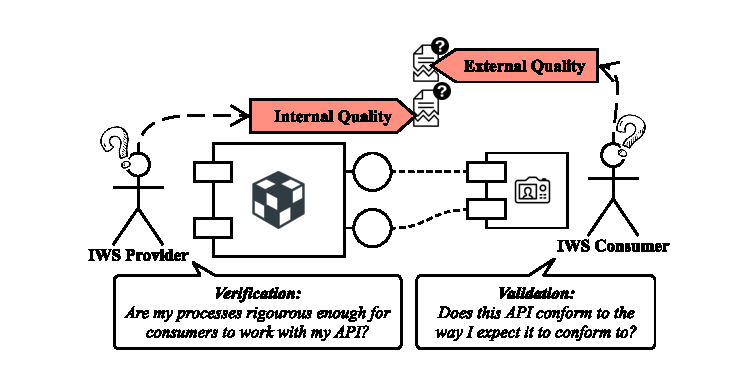
\includegraphics[width=0.8\linewidth]{leakage}
  \caption[Leakage of internal and external quality in CISs]{The `leakage' of internal quality into the API consumer's product and external quality imposing on the API provider.}
  \label{fig:background:software-quality:v-and-v:leakage}
\end{figure}

Therefore, just as the test answers with were both correct and incorrect at the same time, so is the same with \glspl{cis} returning a probabilistic result: no result is certain. While \gls{vv} has been investigated in the area of mathematical and earth sciences for numerical probabilistic models and natural systems \citep{Oreskes:1994gn,Rutten:2004a}, from the software engineering literature, little work has been achieved to look at the surrounding area of probabilistic systems hidden behind \gls{api} calls. 

Now that a developer is using  a probabilistic system behind a deterministic \gls{api} call, what does it mean in the context of \gls{vv}? Do current verification approaches and tools suffice, and if not, how do we fix it? From a validation perspective of \gls{ml} and end-users, after a model is trained and an inference is given and if the output data point is incorrect, how will end users report a defect in the system? Compared to deterministic systems where such tooling as defect reporting forms are filled out (i.e., given input data in a given situation and the output data was X), how can we achieve similar outputs when the system is not non-deterministic? A key problem with the probabilistic mindset is that once a model is `fixed' by retraining it, while one data-point may be fixed, others may now have been effected, thereby not ensuring 100\% validation. Thus, due to the unpredictable and blurry nature of probabilistic systems, \gls{vv} must be re-thought out extensively.

\subsection{Quality Attributes and Models}
\label{ssec:background:software-quality:quality-models}

Similarly, quality models are used to capture internal and external quality attributes via measurable metrics. Is a similar issue reflected from that of \gls{vv} due to nondeterministic systems? As there is no `one' definition of quality, there have been differing perspectives with literature placing varying value on disparate attributes.

\afterpage{
\begin{landscape}
\begin{figure}[p]
  \centering
  \begin{subfigure}[b]{0.49\linewidth}
    \centering
    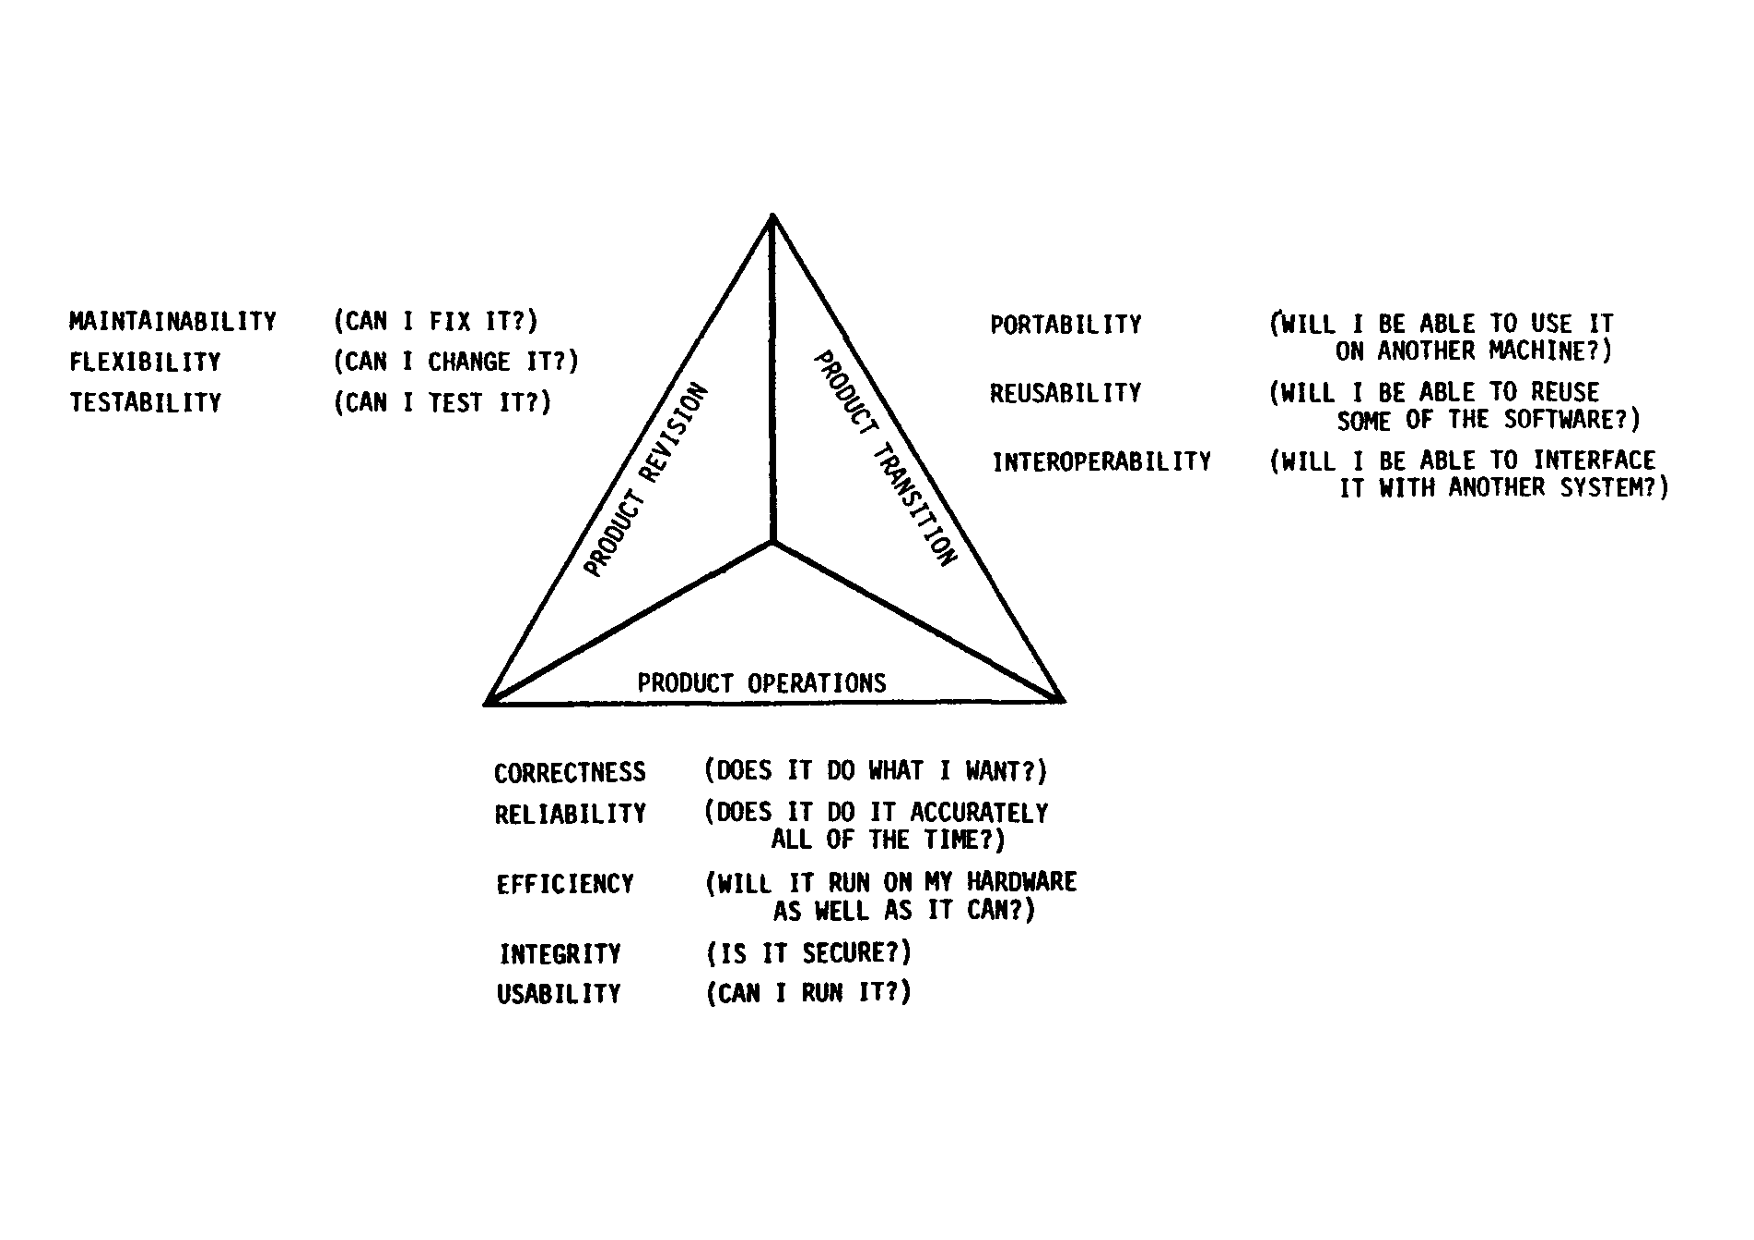
\includegraphics[width=\linewidth]{mcalls-quality-software-factors}
    \caption{McCall's quality software factors (\citeyear{McCall:1977uy}) \citep{McCall:1977uy}.}
    \label{fig:background:software-quality:quality-models:development:mccall}
  \end{subfigure}
  ~
  \begin{subfigure}[b]{0.49\linewidth}
    \centering
    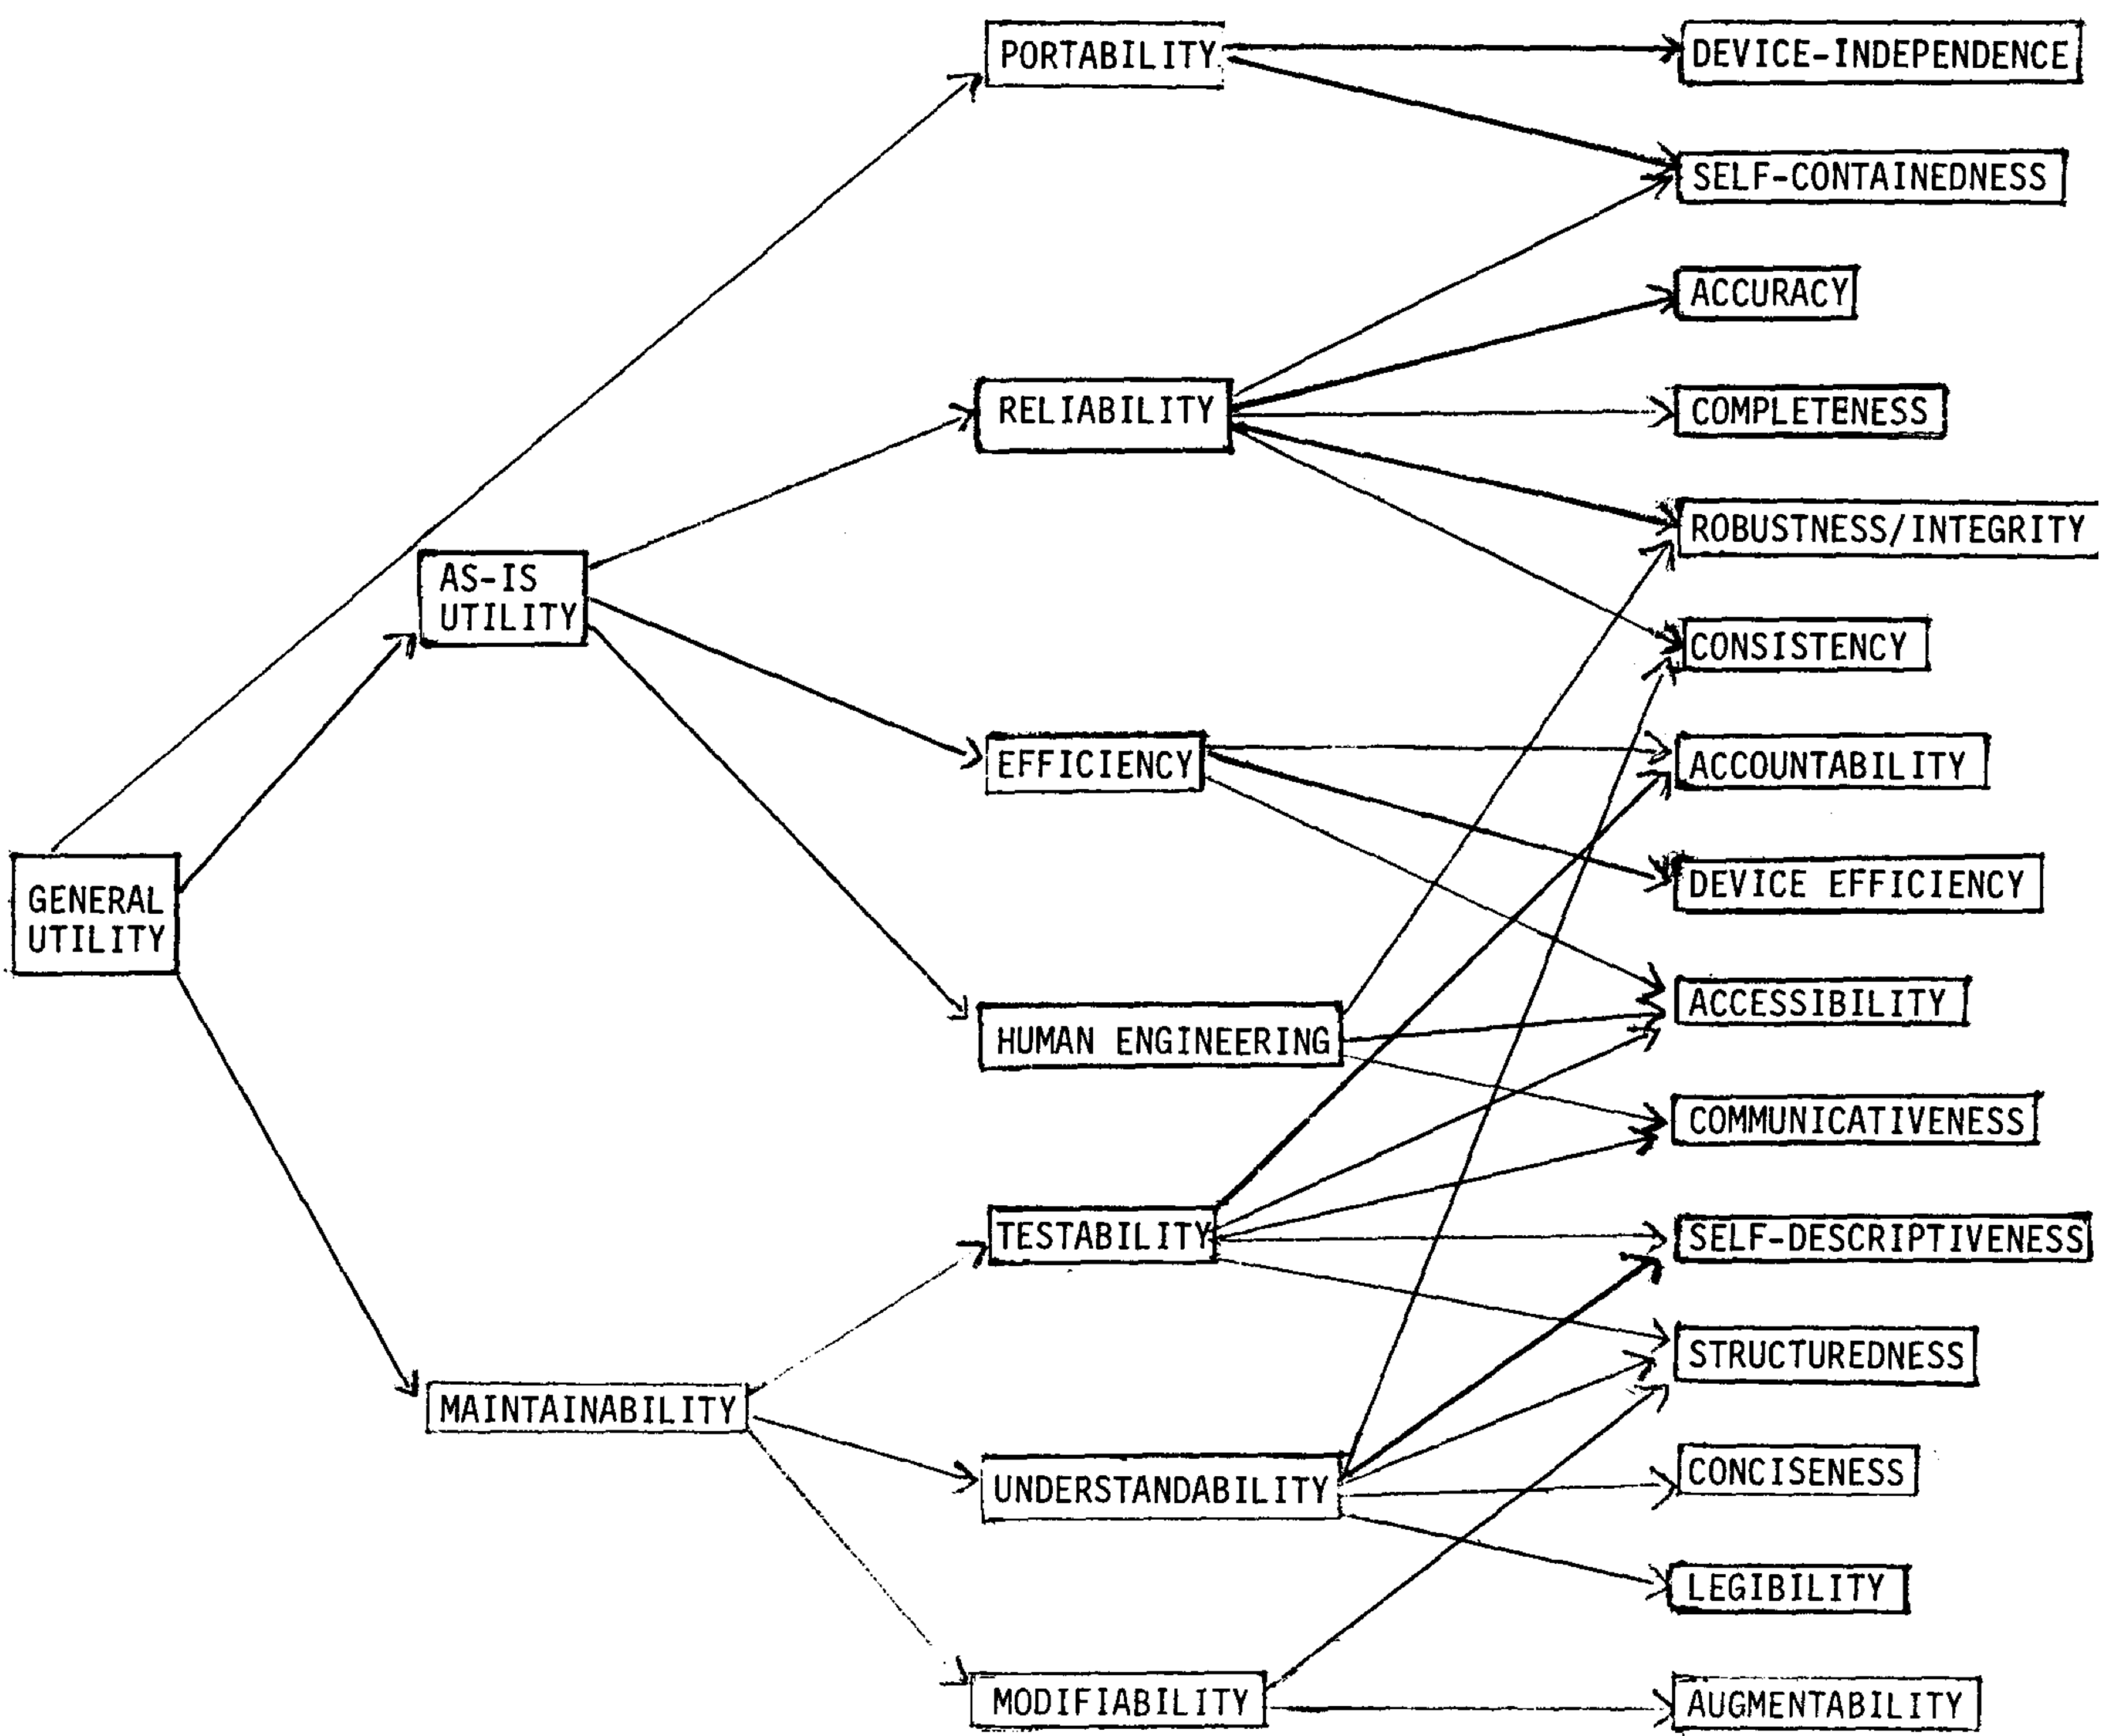
\includegraphics[width=0.7\linewidth]{bohems-software-quality-characteristics-tree}
    \caption{Bohem's software quality characteristics tree (\citeyear{Boehm:1978vv}) \citep{Boehm:1978vv}.}
    \label{fig:background:software-quality:quality-models:development:boehm}
  \end{subfigure}

  \begin{subfigure}[t]{0.49\linewidth}
    \centering
    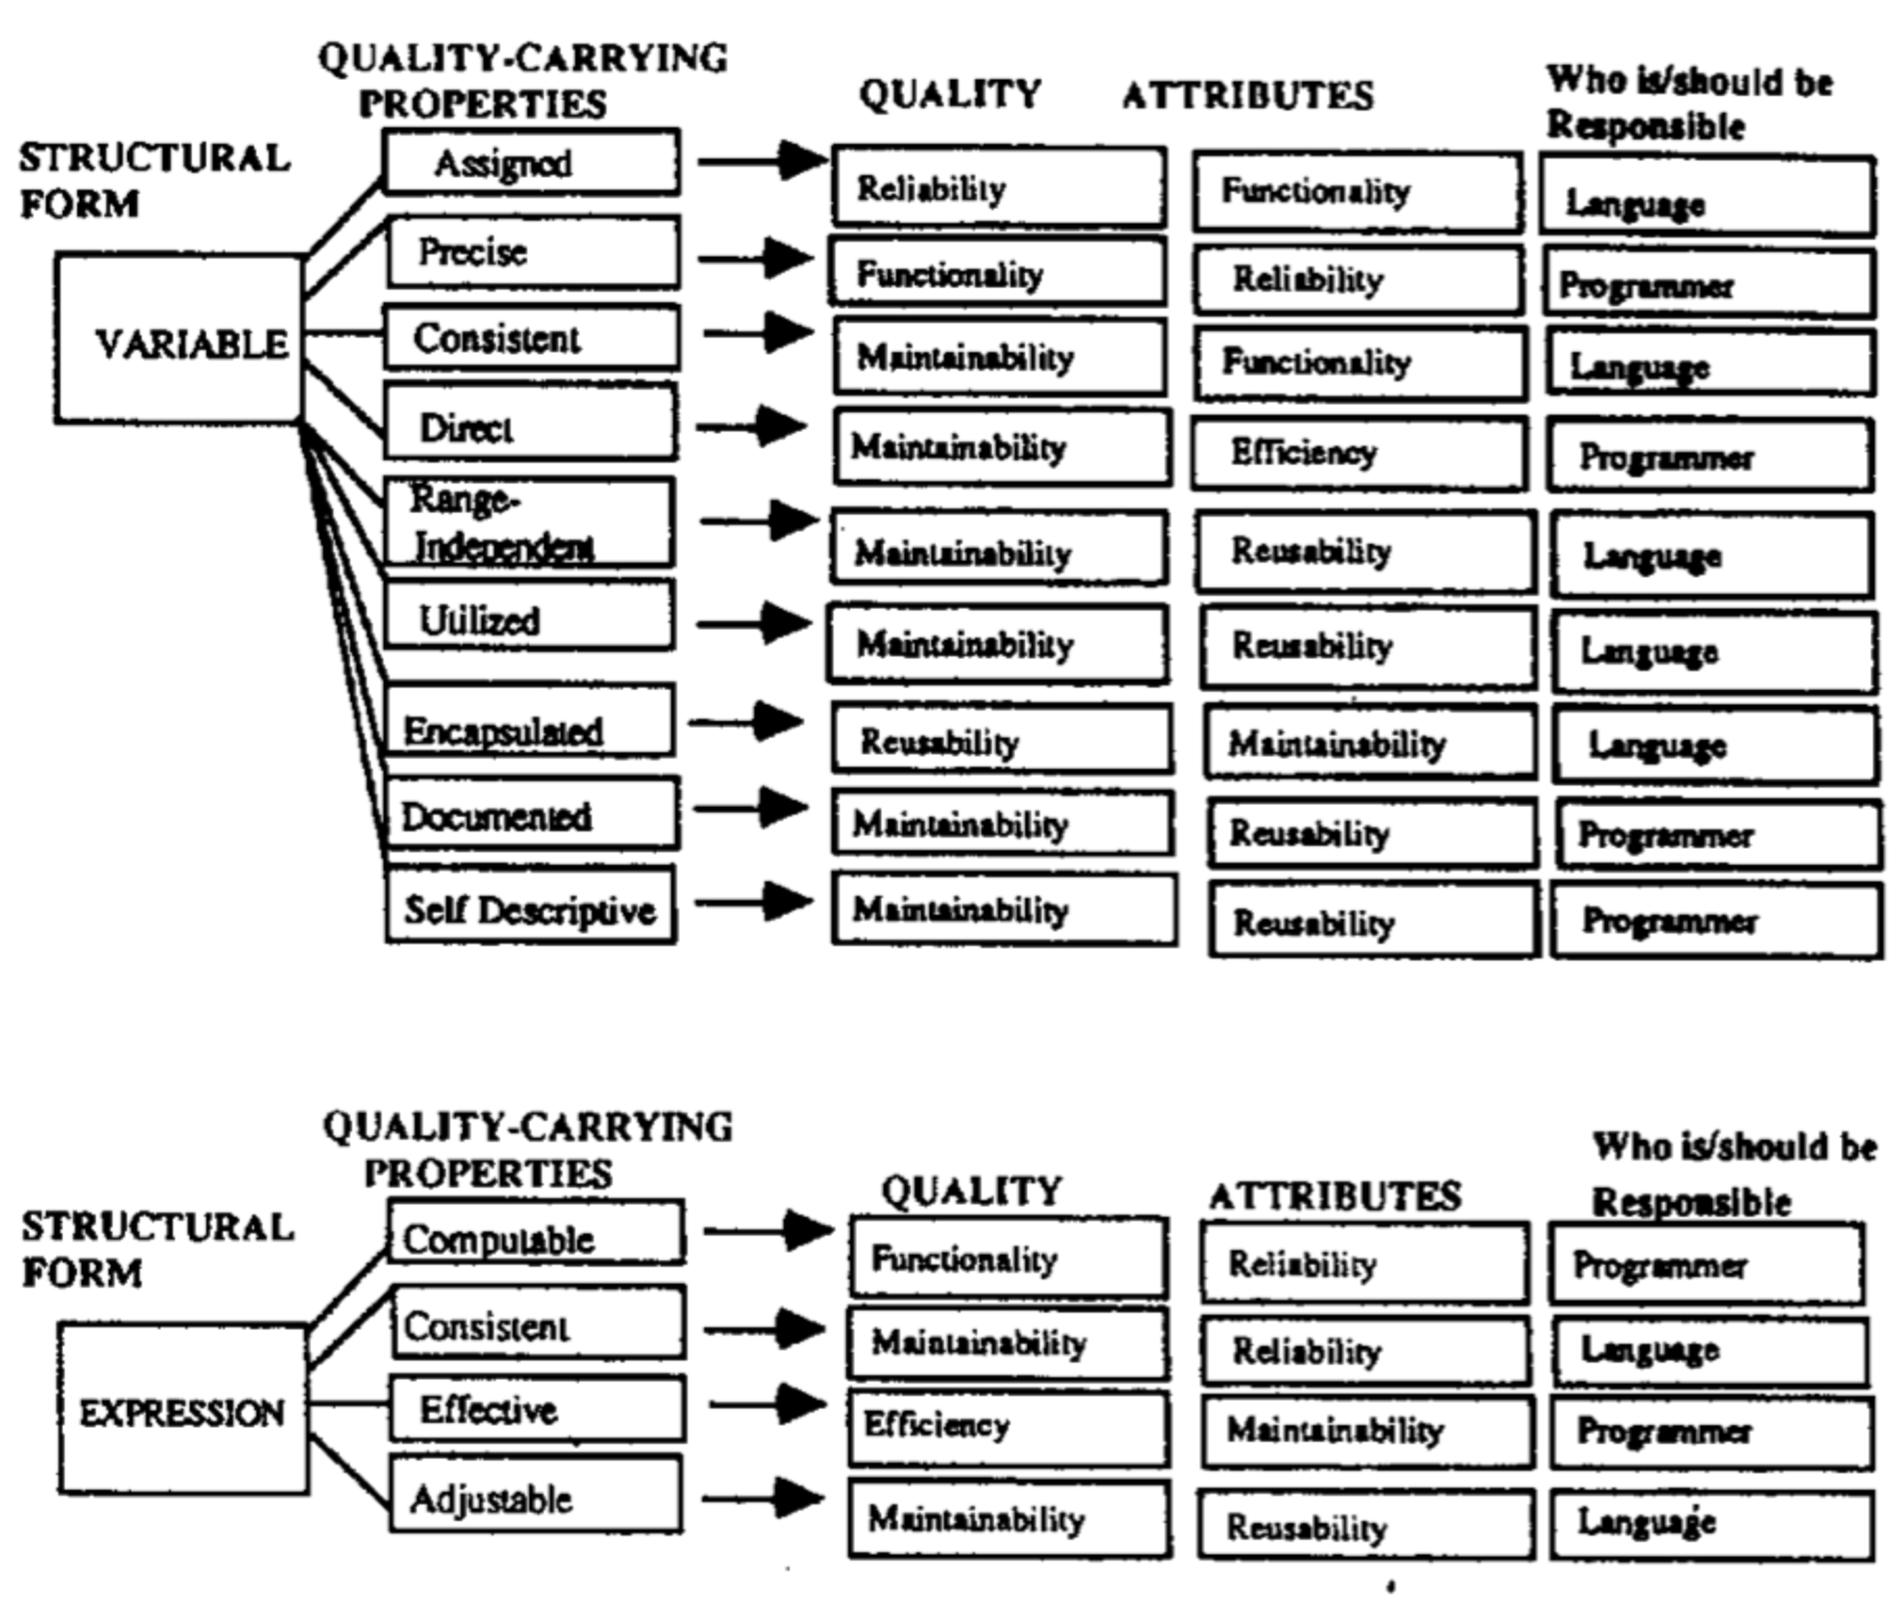
\includegraphics[width=0.6\linewidth]{dromey-quality-carrying-properites}
    \caption{Dromey's quality-carrying properties and programming languages (\citeyear{Dromey:1995wy}) \citep{Dromey:1995wy}.}
    \label{fig:background:software-quality:quality-models:development:dromey}
  \end{subfigure}
  ~
  \begin{subfigure}[t]{0.49\linewidth}
    \centering
    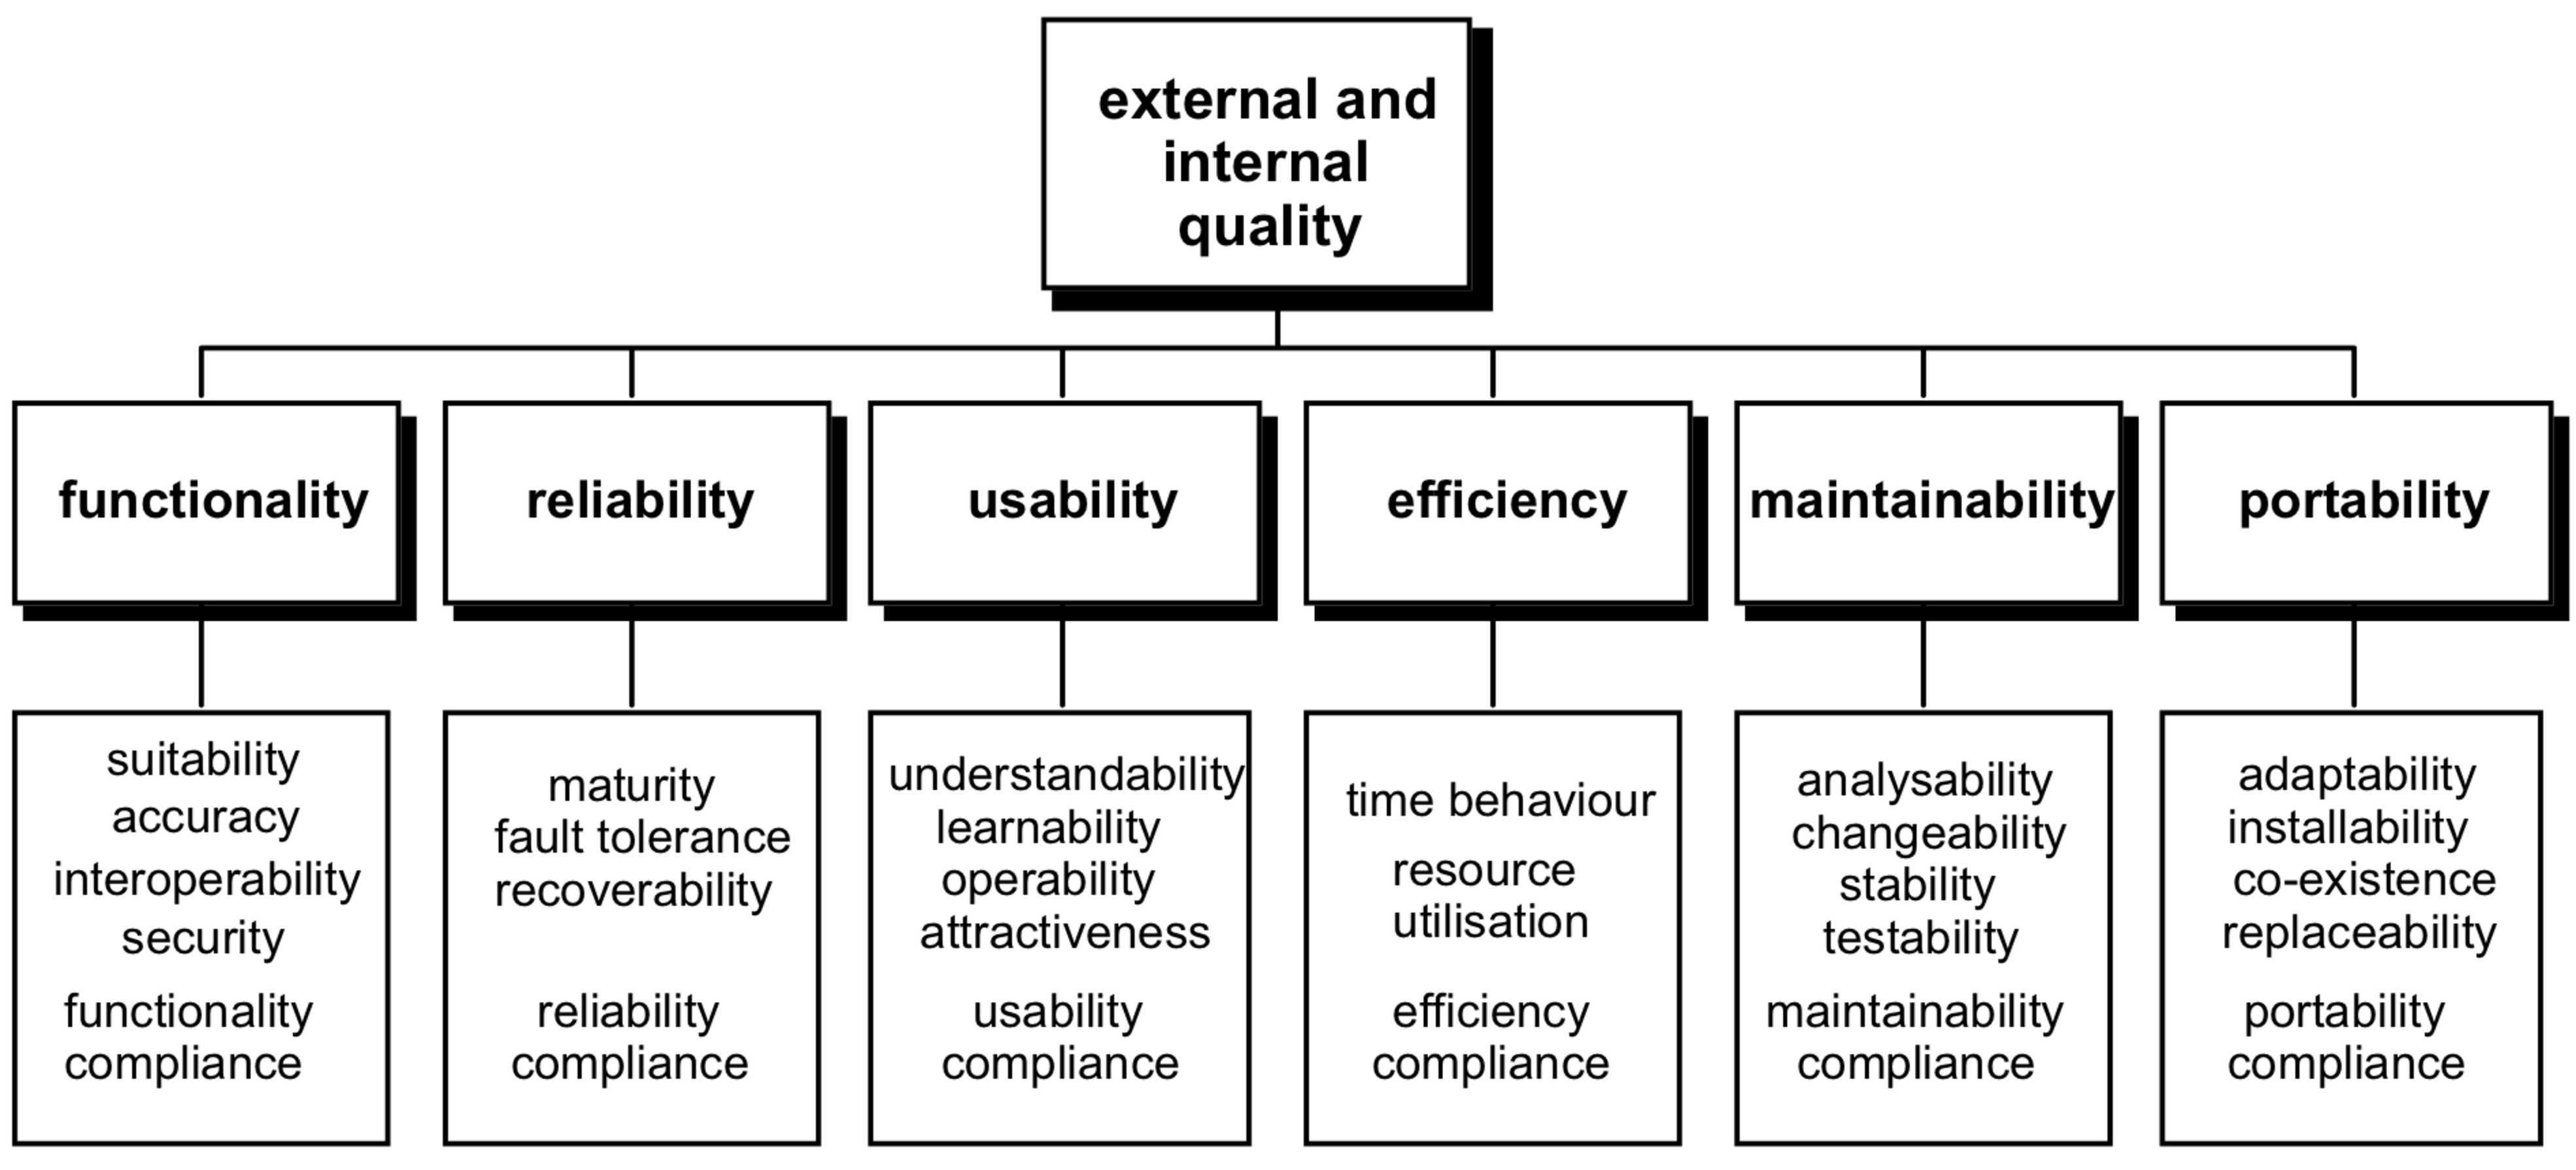
\includegraphics[width=\linewidth]{iso-software-product-evaluation-characteristics}
    \caption{ISO/IEC software product evaluation characteristics (\citeyear{ISO9126:1999}) \citep{ISO9126:1999}.}
    \label{fig:background:software-quality:quality-models:development:iso}
  \end{subfigure}
  \caption[Overview of software quality models]{A brief overview of the development of software quality models since \citeyear{McCall:1977uy}.}
  \label{fig:background:software-quality:quality-models:development}
\end{figure}
\end{landscape}
}

Quality attribute assessment models (like those shown in \cref{fig:background:software-quality:quality-models:development}) are an early concept in software engineering, and systematically evaluating software quality appears as early as \citeyear{Rubey:1968fg} \citep{Rubey:1968fg}. \citeauthor{Rubey:1968fg}'s \citeyear{Rubey:1968fg} study introduced the phrase `attributes' as a ``prose expression of the particular quality of desired software'' (as worded by \citet{Boehm:1978vv}) and `metrics' as mathematical parameters on a scale of 0 to 100. 
Early attempts to categorise wider factors under a framework was proposed by \citeauthor*{McCall:1977uy} in the late 1970s~\citep{McCall:1977wm,Cavano:1978gz}. This model described quality from the three perspectives of product revision (\textit{how can we keep the system operational?}), transition (\textit{how can we migrate the system as needed?}) and operation (\textit{how effective is the system at achieving its tasks?}) (\cref{fig:background:software-quality:quality-models:development:mccall}). The model also introduced 11 attributes alongside numerous direct and indirect measures to help quantify quality.
This model was further developed by \citet{Boehm:1978vv} who independently developed a similar model, starting with an initial set of 11 software characteristics. It further defined candidate measurements of Fortran code to such characteristics, taking shape in a tree-like structure as in \cref{fig:background:software-quality:quality-models:development:boehm}. 
In the mid-1990s, Dromey's interpretation \citep{Dromey:1995wy} defined a set of quality-carrying properties with structural forms associated to specific programming languages and conventions (\cref{fig:background:software-quality:quality-models:development:dromey}). The model also supported quality defect identification and proposed an improved auditing method to automate defect detection for code editors in IDEs. 
As the need for quality models became prevalent, the \citeauthor{ISO9126:1999} standardised software quality under ISO/IEC-9126 \citep{ISO9126:1999} (the Software Product Evaluation Characteristics, \cref{fig:background:software-quality:quality-models:development:iso}), which has since recently been revised to ISO/IEC-25010 with the introduction of the \gls{square} model \citep{ISO25010:2011}, separating quality into \textit{Product Quality} (consisting of eight quality characteristics and 31 sub-characteristics) and \textit{Quality In Use} (consisting of five quality characteristics and 9 sub-characteristics).
An extensive review on the development of quality models in software engineering is given in \citep{AlQutaish:2010vua}.

Of all the models described, there is one quality attribute that relates most with our narrative of \gls{cis} quality: reliability. The definition of reliability is similar among all quality models:

\begin{description}[font=\itshape,style=multiline,leftmargin=3cm]
  \item[\citeauthor{McCall:1977uy}] Extent to which a program can be expected to perform its intended function with required precision \citep{McCall:1977uy}.
  \item[\citeauthor{Boehm:1978vv}] Code possesses the characteristic \textit{reliability} to the extent that it can be expected to perform its intended functions satisfactorily \citep{Boehm:1978vv}.
  \item[\citeauthor{Dromey:1995wy}] Functionality implies reliability. The reliability of software is therefore  dependent on the same properties as functionality, that is, the correctness properties of a program \citep{Dromey:1995wy}.
  \item[ISO/IEC-9126] The capability of the software product to maintain a specified level of performance when used under specified conditions \citep{ISO9126:1999}.
\end{description}

These definitions strongly relate to the system's solution description in that reliability is the ability to maintain its \textit{functionality} under given conditions. But what defines reliability when the nature of a \gls{cis} in itself is inherently unpredictable due to its probabilistic implementation? Can a non-deterministic system ever be considered reliable when the output of the system is uncertain? How do developers perceive these quality aspects of reliability in the context of such systems? A system cannot be perceived as `reliable' if the system cannot reproduce the same results due to a probabilistic nature. Therefore, we believe the literature of quality models does not suffice in the context of \gls{cis} reliability; a \gls{cvcis} can interpret an image of a dog as a `Dog' one day, but what if the next it interprets such image more specifically to the breed, such as `Border Collie'? Does this now mean the system is unreliable? 

Moreover, defining these systems in themselves is challenging when requirements specifications and solution descriptions are dependent on nondeterministic and probabilistic algorithms. We discuss this further in \cref{sec:background:probabilistic-stochastic}.

\subsection{Reliability in Computer Vision}
\label{ssec:background:software-quality:reliability-in-cv}

Testing computer vision deep-learning reliability is an area explored typically through the use of adversarial examples \citep{Szegedy:2013vw}. These input examples are where images are slightly perturbed to maximise prediction error but are still interpretable to humans. Refer to \cref{fig:background:software-quality:reliability-in-cv:adversarial-examples}.

\begin{figure}[p]
  \centering
  \begin{subfigure}[b]{0.4\linewidth}
    \centering
    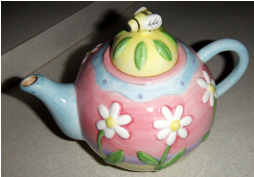
\includegraphics[width=\linewidth]{adversarial-teapot-org}\\
    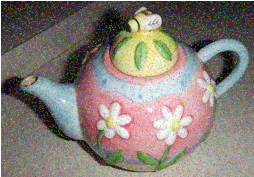
\includegraphics[width=\linewidth]{adversarial-teapot-noisy}
    \caption{Adding 10\% impulse noise to an image of a teapot changes Google Cloud Vision's label from \textit{teapot} (above) to \textit{biology} (below) \citep{Hosseini:2018jr}.}
  \end{subfigure}
  ~
  \begin{subfigure}[b]{0.4\linewidth}
    \centering
    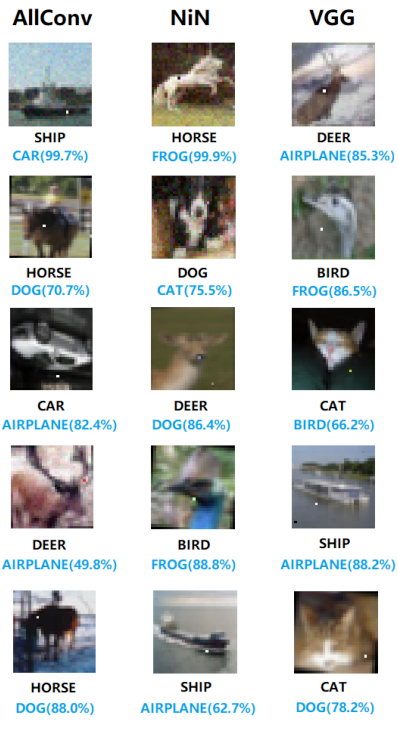
\includegraphics[width=\linewidth]{adversarial-one-pixel}
    \caption{One-pixel attacks applied to three \gls{nn}: AllConv, NiN and VGG \citep{Su:2017uw}.}
  \end{subfigure}
  \\ \bigskip
  \begin{subfigure}[b]{0.8\linewidth}
    \centering
    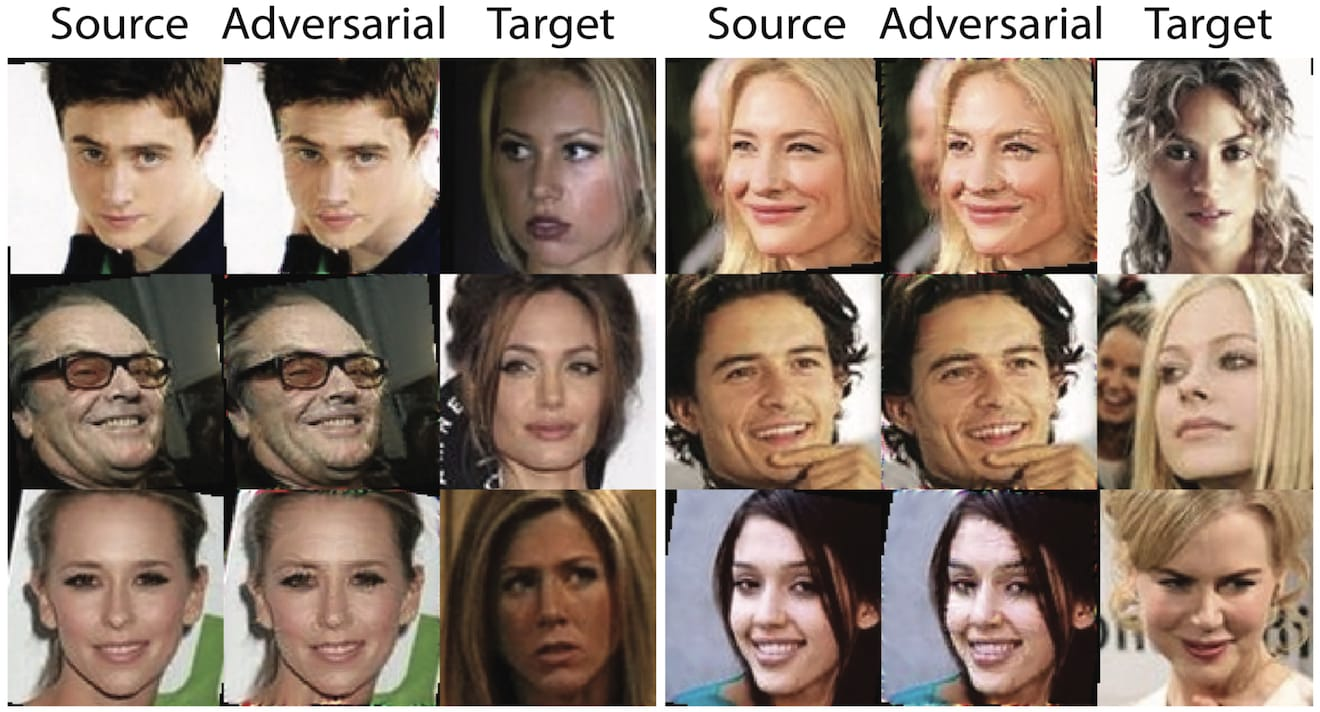
\includegraphics[width=\linewidth]{adversarial-celebrities}
    \caption{Adversarial examples to trick face recognition from the source to target images \citep{Wang:2018vl}.}
  \end{subfigure}

  \caption[Sample adversarial examples]{Sample adversarial examples.}
  \label{fig:background:software-quality:reliability-in-cv:adversarial-examples}
\end{figure}

Google Cloud Vision, for instance, fails to correctly classify adversarial examples when noise is added to the original images \citep{Hosseini:2018jr}. \citet{Rosenfeld:2018ut} illustrated that inserting synthetic foreign objects to input images (e.g., a cartoon elephant) can alter classification output. \citet{Wang:2018vl} performed similar attacks on a transfer-learning approach of facial recognition by modifying pixels of a celebrity's face to be recognised as a different celebrity, all while still retaining the same human-interpretable original celebrity. \citet{Su:2017uw} used the ImageNet database to show that 41.22\% of images drop in confidence when just a \textit{single pixel} is changed in the input image; and similarly, \citet{Eykholt:2018vka} recently showed similar results that made a \gls{cnn} interpret a stop road-sign (with mimiccid graffiti) as a 45mph speed limit sign.

Thus, the state-of-the-art computer vision techniques may not be reliable enough for safety critical applications (such as self-driving cars) as they do not handle intentional or unintentional adversarial attacks. Moreover, as such adversarial examples exist in the physical world \citep{Kurakin:2016vw,Eykholt:2018vk}, ``the real world may be adversarial enough'' \citep{Pezzementi:2018tq} to fool such software.

\section{Probabilistic and Nondeterministic Systems}
\label{sec:background:probabilistic-stochastic}

Probabilistic and nondeterministic systems are those by which, for the same given input, different outcomes may result. The underlying models that power an \gls{iws} are treated as though they are nondeterministic; \cref{ch:background} introduces \glspl{iws} as essentially black-box behaviour that can change over time. As such, we adopt the nondeterministic behaviour that they present.

\begin{figure}[h!]
  \centering
  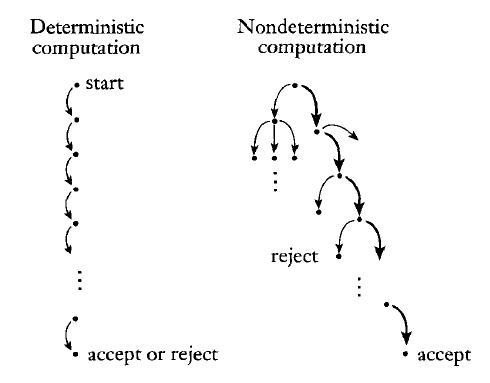
\includegraphics[width=0.6\linewidth]{nfa-compute}
  \caption[Deterministic versus nondeterministic systems]{A deterministic system (left) always returns the same result in the same amount of steps. A nondeterministic system does not guarantee the same outcome, even with the same input data. Source:~\citep{Finalyson:2018aa}.}
  \label{fig:background:probabilistic-stochastic:nfa-compute}
\end{figure}

\subsection{Interpreting the Uninterpretable}
\label{ssec:background:probabilistic-stochastic:model-interpretability}

As the rise of applied \gls{ai} increases, the need for engineering interpretability around models becomes paramount, chiefly from an external quality perspective that the \textit{reliability} of the system can be inspected by end-users. Model interpretability has been stressed since early machine learning research in the late 1980s and 1990s (such as \citet{Quinlan:1999ue} and \citet{Michie:1988te}), and although there has since been a significant body of work in the area \citep{Singh:2016wu,Baehrens:2010tj,Ribeiro:2016gg,Bussone:2015wm,Ross:2017vn,Lipton:2016if,Boz:2002uv,Johansson:2009uo,Augasta:2012wx,Fung:2005we,Dejaeger:2012up,VanAssche:2007wc,BenDavid:1995up,Feelders:2000ve,Lima:2009tm,Martens:2011uh,Pazzani:1997vp,Verbeke:2011vo}, it is evident that `accuracy' or model `confidence' is still used as a primary criterion for AI evaluation \citep{Huang:2005tc,Japkowicz:2011vy,Sokolova:2009vu}. Much research into \glsx{nn} or \glsx{svm} development stresses that `good' models are those with high accuracy. However, is accuracy enough to justify a model's quality?

To answer this, we revisit what it means for a model to be accurate. Accuracy is an indicator for estimating how well a model's algorithm will work with future or unforeseen data. It is quantified in the \gls{ai} testing stage, whereby the algorithm is tested against cases known by humans to have ground truth but such cases are unknown by the algorithm. In production, however, all cases are unknown by both the algorithm \textit{and} the humans behind it, and therefore a single value of quality is ``not reliable if the future dataset has a probability distribution significantly different from past data'' \citep{Freitas:2014ic}, a problem commonly referred to as the \textit{datashift} problem \citep{Sugiyama:2017ud}. Analogously, \citet{Freitas:2014ic} provides the following description of the problem:

\begin{quote}
\itshape
The military trained [a \gls{nn}] to classify images of tanks into enemy and friendly tanks. However, when the [\gls{nn}] was deployed in the field (corresponding to ``future data''), it had a poor accuracy rate. Later, users noted that all photos of friendly (enemy) tanks were taken on a sunny (overcast) day. I.e., the [\gls{nn}] learned to discriminate between the colors of the sky in sunny vs. overcast days! \textbf{If the [\gls{nn}] had output a comprehensible model (explaining that it was discriminating between colors at the top of the images), such a trivial mistake would immediately be noted.}
\upshape
\citep{Freitas:2014ic}
\end{quote}

So, why must we interpret models? While the formal definition of what it means to be \textit{interpretable} is still somewhat disparate (though some suggestions have been proposed \citep{Lipton:2016if}), what is known is (i) there exists a critical trade-off between accuracy and interpretability \citep{Freitas:2004vv,Jin:2006uf,Kaufman:1999vg,Grunwald:2007vg,Domingos:1998ug,Zahalka:2011ux}, and (ii) a single quantifiable value cannot satisfy the subjective needs of end-users \citep{Freitas:2014ic}. As ever-growing domains \gls{ml} become widespread\footnote{In areas such as medicine \citep{Bellazzi:2008tv,Lavrac:1999tf,Pazzani:2001tw,Richards:2001vw,Zupan:2000tp,VanAssche:2007wc,Johansson:2009uo,Elazmeh:2007tp,Wong:2006ve,Jaspers:2011hy,Bussone:2015wm}, bioinformatics \citep{Freitas:2010vk,Szafron:2004uf,Karwath:2002tv,Doderer:2006vt,Jiang:2005ua}, finance \citep{Baehrens:2010tj,Huysmans:2011gq,Dhar:2000vo} and customer analytics \citep{Verbeke:2011vo,Lima:2009tm}.}, these applications engage end-users for real-world goals, unlike the aims in early \gls{ml} research where the aim was to get \gls{ai} working in the first place. In safety-critical systems where \gls{ai} provide informativeness to humans to make the final call (see \citep{Caruana:2015jk,Kim:2015vo,Huysmans:2011gq}), there is often a mismatch between the formal objectives of the model (e.g., to minimise error) and complex real-world goals, where other considerations (such as the human factors and cognitive science behind explanations\footnote{\textit{Interpretations} and \textit{explanations} are often used interchangeably.}) are not realised: model optimisation is only worthwhile if they ``actually solve the original [human-centred] task of providing explanation'' \citep{Narayanan:2018ud} to end-users. \textbf{Therefore, when human-decision makers must be interpretable themselves \citep{Ridgeway:1998ud}, any \gls{ai} they depend on must also be interpretable.} 

Recently, discussion behind such a notion to provide legal implications of interpretability is topical. \citet{DoshiVelez:2017vm} discuss when explanations are not provided from a legal stance---for instance, those affected by algorithmic-based decisions have a `right to explanation' \citep{Goodman:2016wf,Wachter:2017hx} under the European Union's GDPR\footnoteurl{https://www.eugdpr.org}{13 August 2018}. But, explanations are not the only way to ensure \gls{ai} accountability: theoretical guarantees (mathematical proofs) or statistical evidence can also serve as guarantees \citep{DoshiVelez:2017vm}, however, in terms of explanations, what form they take and how they are proven correct are still open questions \citep{Lipton:2016if}.

\subsection{Explanation and Communication}
\label{ssec:background:probabilistic-stochastic:communication}

From a software engineering perspective, explanations and interpretability are, by definition, inherently communication issues: what lacks here is a consistent interface between the \gls{ai} system and the person using it. The ability to encode `common sense reasoning' \citep{McCarthy:1960:PCS:889202} into programs today has been achieved, but \textit{decoding} that information is what still remains problematic. At a high level, \citeauthor{Shannon:1963ti}'s theory of communication \citep{Shannon:1963ti} applies, just as others have done with similar issues in the software engineering realm \citep{Moody:2009vo,Wickham:2010hy} (albeit to the domain of visual notations). Humans map the world in higher-level concepts easily when compared to \gls{ai} systems: while we think of a tree first (not the photons of light or atoms that make up the tree), an algorithm simply sees pixels, and not the concrete object \citep{DoshiVelez:2017vm} and the \gls{ai} interprets the tree inversely to humans. Therefore, the interpretation or explanation is done inversely: humans do not explain the individual neurons fired to explain their predictions, and therefore the algorithmic transparent explanations of \gls{ai} algorithms (\textit{``which neurons were fired to make this \gls{ai} think this tree is a tree?''}) do not work here.

Therefore, to the user (as mapped using \citeauthor{Shannon:1963ti}'s theory), an AI pipeline (the communication \textit{channel}) begins with a real-world concept, $y$, that acts as an \textit{information source}. This information source is fed in as a \textit{message}, $x$, (as pixels) to an AI system (the \textit{transmitter}). The transmitter encodes the pixels to a prediction, $\hat{y}$, the \textit{signal} of the message. This signal is decoded by the \textit{receiver}, an explanation system, $e_{x}(x,\hat{y})$, that tailors the prediction with the given input data to the intended end user (the \textit{destination}) as an explanation,~$\tilde{y}$, another type of \textit{message}. Therefore, the user only sees the channel as an input/output pipeline of real-world objects, $y$, and explanations, $\tilde{y}$, tailored to \textit{them}, without needing to see the inner-mechanics of a prediction $\hat{y}$. We present this diagrammatically in \cref{fig:background:probabilistic-stochastic:theory-of-ai-communication}.

\begin{figure}[t!]
  \centering
  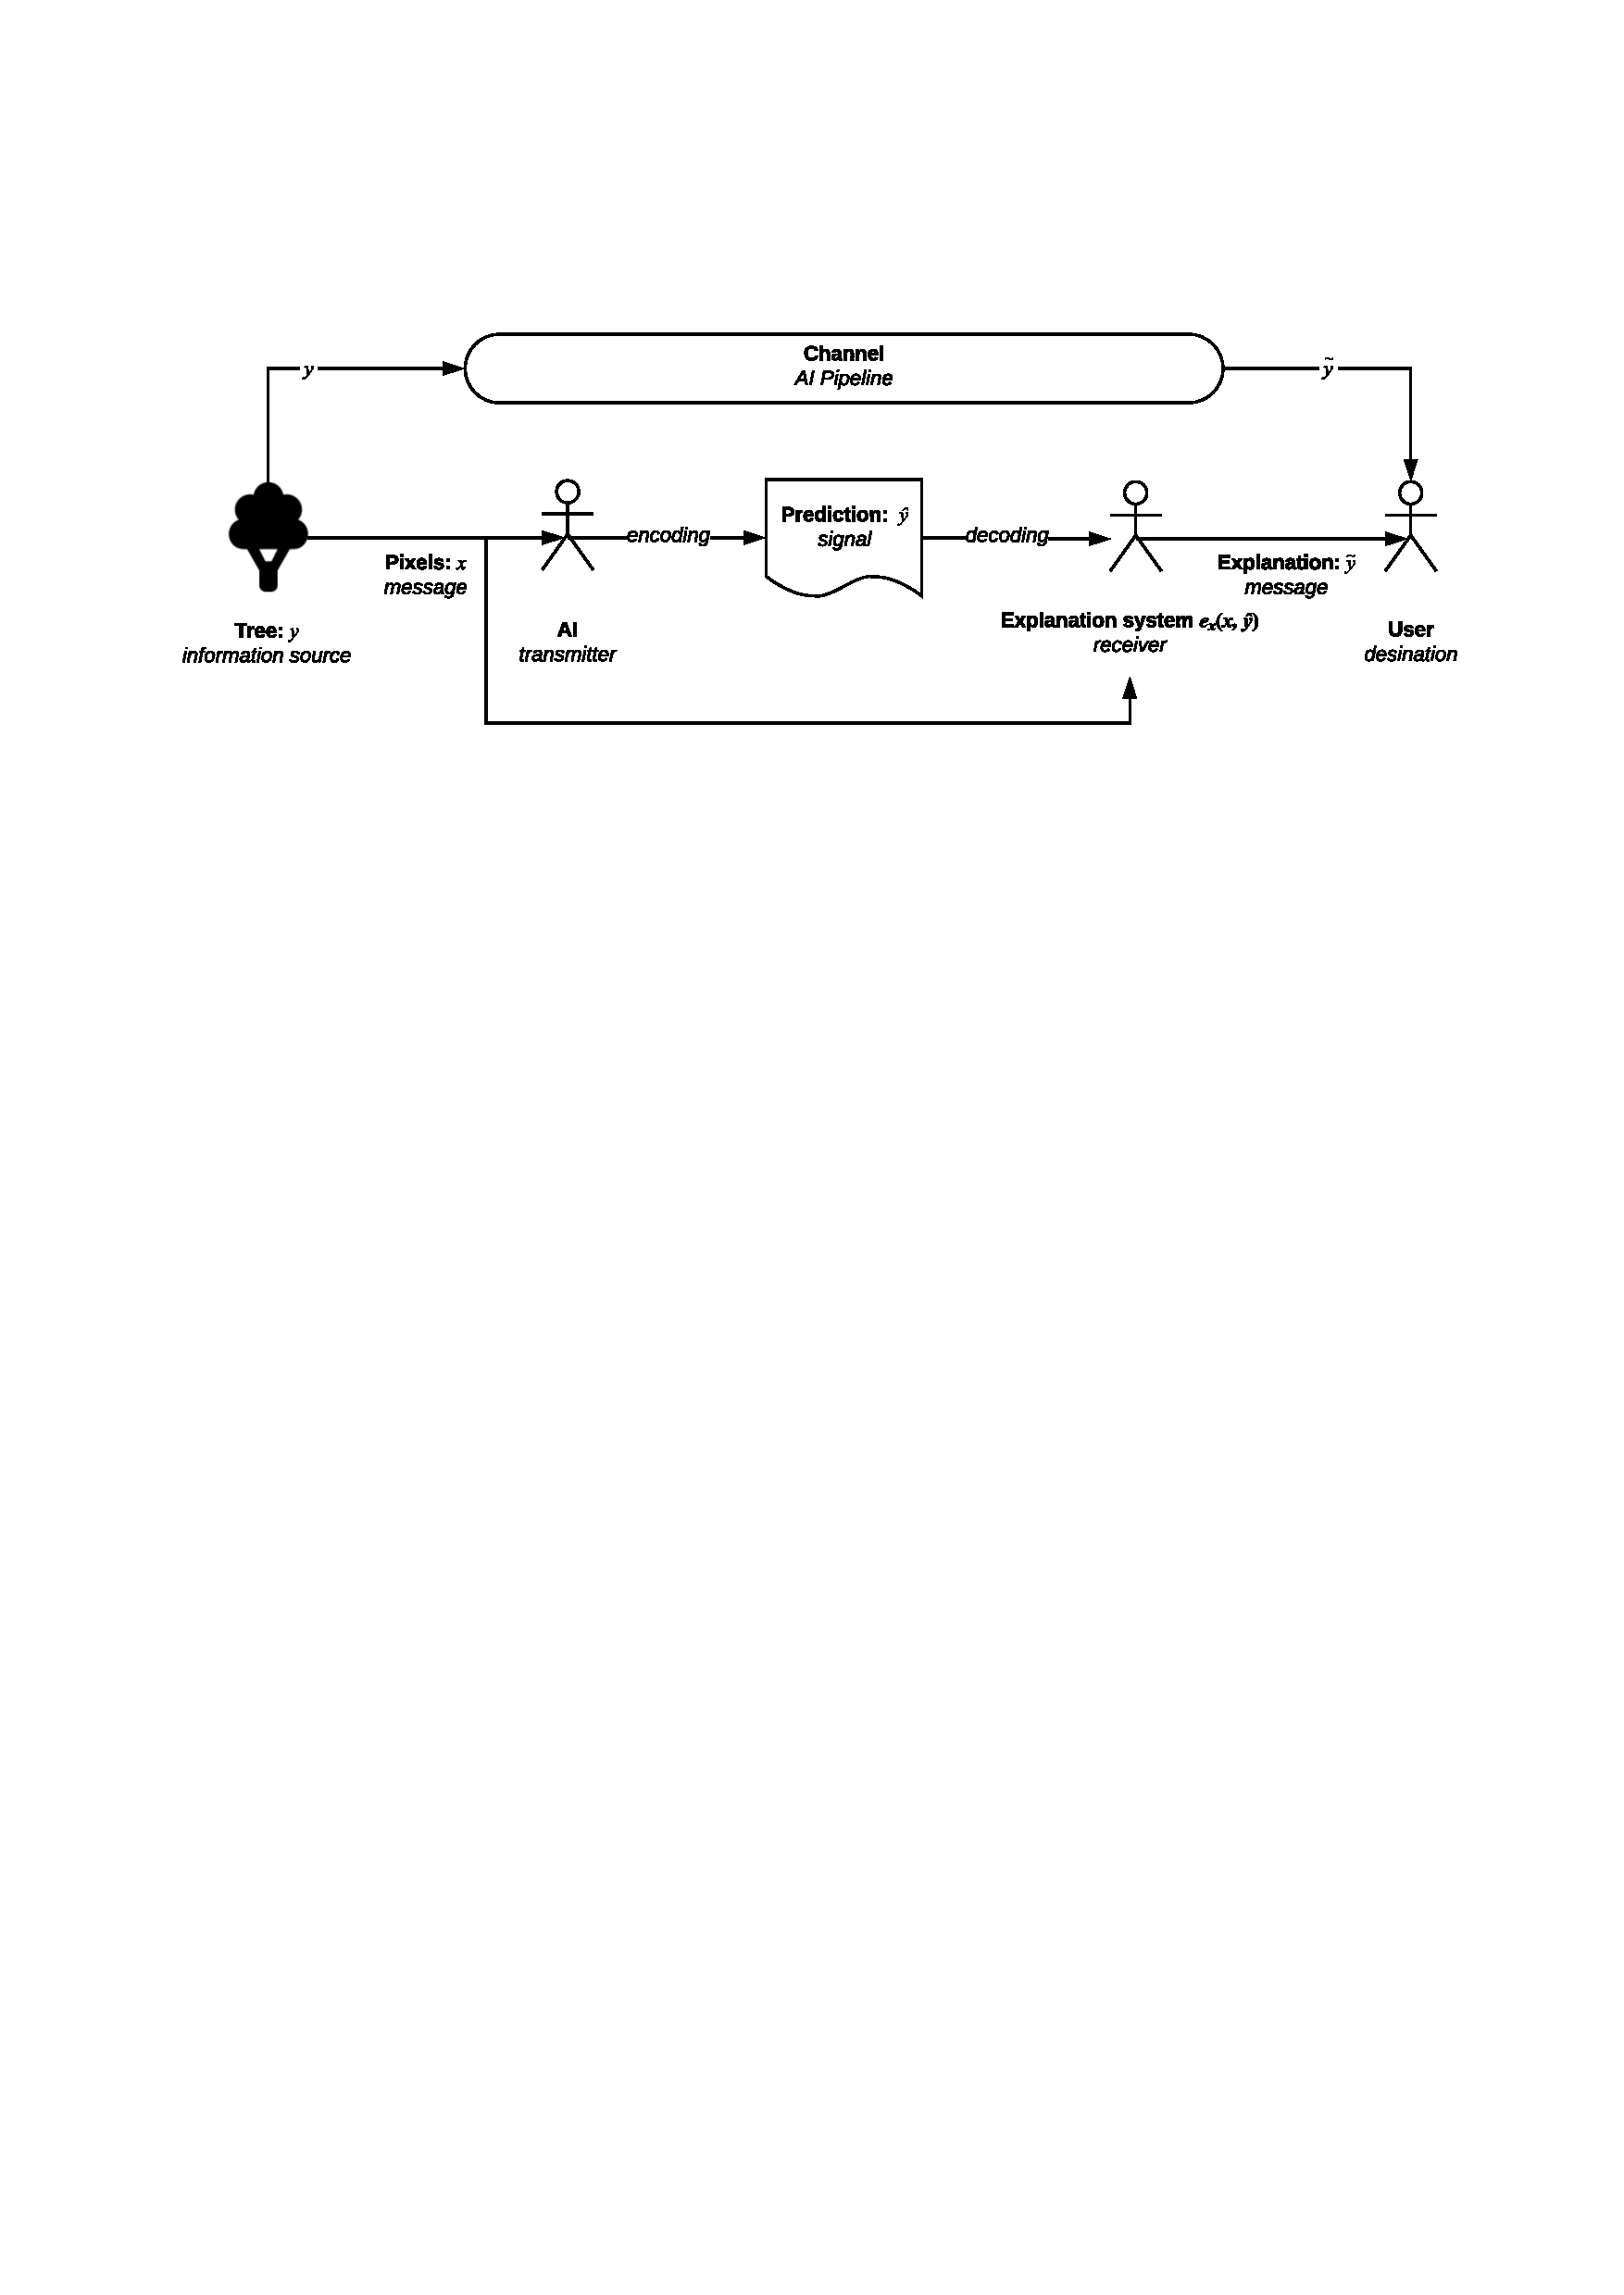
\includegraphics[width=\textwidth]{communication}
  \caption[Theory of AI communication]{Theory of AI communication from information source, $y$, to intended user as explanations, $\tilde{y}$.}
  \label{fig:background:probabilistic-stochastic:theory-of-ai-communication}
\end{figure}

\subsection{Mechanics of Model Interpretation}
\label{ssec:background:probabilistic-stochastic:mechanics}

How do we interpret models? Methods for developing interpretation models include: decision trees \citep{Breiman:1984tu,Hastie:2001wp,Craven:1995wg,Quinlan:1993vi,Rokach:2008wc}, decision tables \citep{Lima:2009tm,Baesens:2003we} and decision sets \citep{Lakkaraju:2016ka,Narayanan:2018ud}; input gradients, gradient vectors or sensitivity analysis \citep{Selvaraju:2017bk,Ribeiro:2016gg,Lei:2016wi,Ross:2017vn,Baehrens:2010tj}; exemplars \citep{Kim:2014ui,Frey:2007hs}; generalised additive models \citep{Caruana:2015jk}; classification (\textit{if-then}) rules \citep{Thrun:1996wh,Bramer:2007vg,Clark:1991vi,Otero:2013ul,Witten:2016ut} and falling rule lists \citep{Singh:2016wu}; nearest neighbours \citep{Martens:2011uh,Sen:1995uk,Suri:2007wl,Wettschereck:1997vw,Zhang:2008vfa} and Na\"{i}ve Bayes analysis \citep{Bellazzi:2008tv,Lavrac:1999tf,Kononenko:1993td,Zupan:2000tp,Michie:1994wi,Friedman:1997vs,Cheng:2001vw,Heckerman:2000uw}. 

Cross-domain studies have assessed the interpretability of these techniques against end-users, measuring response time, accuracy in model response and user confidence \citep{Huysmans:2011gq,Hayete:2005tn,Allahyari:2011ud,Subramanian:1992ue,Schwabacher:2001wc,Freitas:2010vk,Martens:2011uh,Verbeke:2011vo}, although it is generally agreed that decision rules and decision tables provide the most interpretation in non-linear models such as \glspl{svm} or \glspl{nn} \citep{Freitas:2010vk,Martens:2011uh,Verbeke:2011vo}. For an extensive survey of the benefits and fallbacks of these techniques, we refer to \citet{Freitas:2014ic}, \citet{DoshiVelez:2017vm} and \citet{DoshiVelez:2017wu}.

An important factor in model interpretation is to avoid over-reliance, and thus, one mechanism of model interpretation is to reduce explanations  altogether. For example, \citet{Bussone:2015wm} showed that, in clinical decision support systems, confidence values alone only results in a slight effect on trust and reliance of a system. However, having overly detailed explanations may also cause over-reliance on systems if explanations are detailed but not necessarily true \citep{Bussone:2015wm}. Hence, a mechanism of model interpretation for the purpose of ensuring trust and reliance is to deliberately show \textit{fewer} explanations or \textit{incorrect} explanations, thereby avoiding over-reliance. A balance between under-explained and overly-explained models is required. This is to encourage intuition in users of a system; similarly, in \citet{Ribeiro:2016gg}, it was shown that accuracy alone is not always the best way to ascertain trust. Thus, intuitive factors are also mechanisms that can be encoded into explainable models.

\section{Application Programming Interfaces}

\glsplx{api} are the interface between a developer needs and the software components at their disposal \citep{Arnold:2005vc} by abstracting the underlying component behind a subroutine, protocol or specific tool. Therefore, it is natural to assess internal quality (and external quality if the software is in itself a service to be used by other developers---in this case a \gls{cis}) is therefore directly related to the quality the \gls{api} offers \citep{Ko:2004td}. 

Good \glspl{api} are known to be intuitive and require less documentation browsing \citep{Piccioni:2013em}, thereby increasing developer productivity. Conversely, poor APIs are those that are hard to interpret, thereby reducing developer productivity and product quality. The consequences of this have shown a higher demand of technical support (as measured in \citep{Henning:2009hz}) that, ultimately, causes the maintenance to be far more expensive, a phenomenon widely known in software engineering economics (see \cref{ssec:background:software-quality:v-and-v}).

While there are different types of \glspl{api}, such as software library/framework \glspl{api} for building desktop software, operating system \glspl{api} for interacting with the operating system, remote \glspl{api} for communication of varying technologies through common protocols, we focus on web \glspl{api} for communication of resources over the web (being the common architecture of cloud-based services).

\subsection{The Development, Documentation and Usage of Web APIs}

The development of web \glspl{api} (commonly referred to as a \textit{web service}) and web \glspl{api} traces its roots back to the early 1990s, where  the Open Software Foundation's \gls{dce} introduced a collection of services and tools for developing and maintaining distributed systems using a client/server architecture \citep{Rosenberry:1992up}. This framework used the synchronous communication paradigm \glspl{rpc} first introduced by \citet{Nelson:1981ue} that allows procedures to be called in an remote address space as if it were local. Its communication paradigm, \gls{dce}/\gls{rpc} \citep{OpenSoftwareFoundation:1991vp}, enables developers to write distributed software with underlying network code abstracted away. To bridge remote \gls{dce}/\glspl{rpc} over components of different operating systems and languages, a \gls{idl} document served as the common service contract or \textit{service interface} for software components. 

This important leap toward language-agnostic distributed programming paved way for \glsac{xml}-\gls{rpc}, enabling \glspl{rpc} over \glsac{http} (and thus the Web) encoded using \glsac{xml} (instead of octet streams \citep{OpenSoftwareFoundation:1991vp}). As new functionality was introduced, this lead to the natural development of the \gls{soap}, the backbone messaging connector for \gls{ws} applications, a realisation of the \gls{soa} \citep{Casati:2003vi} pattern. The \gls{soa} pattern prescribes that services are offered by service providers and consumed by service consumers in a platform- and language-agnostic manner and are used in large-scale enterprise systems (e.g., banking, health). Key to the \gls{soa} pattern is that a service's quality attributes (see \cref{sec:background:software-quality}) can be specified and guaranteed using a \gls{sla} whereby the consumer and provider agree upon a set level of service, which in some cases are legally binding \citep{Bass:2003wi}. This agreement can be measured using \gls{qos} parameters met by the service provider during the transportation layer (e.g., response time, cost of leasing resources, reliability guarantees, system availability and trust/security assurance \citep{Hwang:2017tr,Weerawarana:2005wx}) and these are included within \gls{soap} headers; thus, \gls{qos} aspects are independent from the transport layer and instead exist at the application layer \citep{Pautasso:2008uw}. The \gls{idl} of \gls{soap} is \gls{wsdl}, providing a description of how the web service is invoked, what parameters to expect, and what data structures are returned.

\begin{figure}[h!]
  \centering
  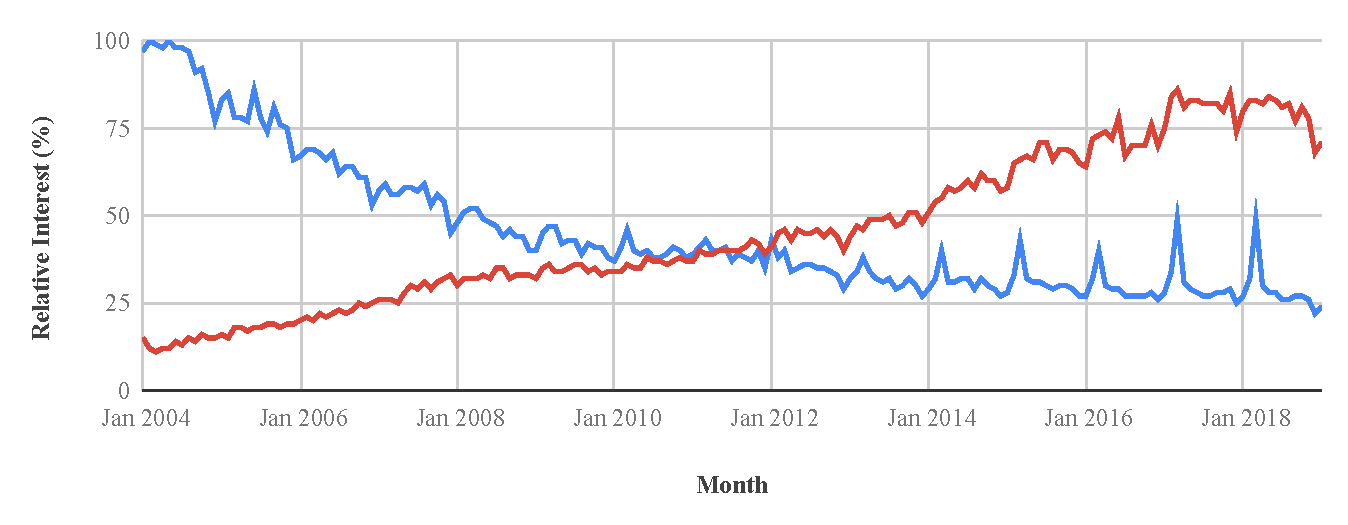
\includegraphics[width=\linewidth]{rest-vs-soap}
  \caption[SOAP versus REST search interest over time]{Worldwide search interest for \glsac{soap} (blue) and \glsac{rest} (red) since 2004. Source:~\citep{Anonymous:Ey7UCSJb}}
  \label{fig:background:apis:rest-vs-soap}
\end{figure}

While it is rich in metadata and verbosity, discussions on whether this was a benefit or drawback came about the mid-2000s \citep{zurMuehlen:2005ci,Pautasso:2008uw} whether the amount of data transfer paid off (especially for mobile clients where data usage was scarce). Developer usability for debugging the \gls{soap} `envelopes' (messages POSTed over \glsac{http} to the service provider component) was difficult, both due to the nature of \glsac{xml}'s wordiness and difficulty to test (by sending POST requests) in-browser. As a simple example, 25 lines (794 bytes) of \glsac{http} communication is transferred to request a customer's name from a record using \gls{soap} (\cref{lst:background:apis:soap-request,lst:background:apis:soap-response}). 

\gls{soap} uses the architectural principle that web services (or the applications they provide) should remain \textit{outside} the web, using \glsac{http} only as a tunnelling protocol to enable remote communication \citep{Pautasso:2008uw}. That is, the \glsac{http} is considered as a transport protocol solely. In 2000, \citet{Fielding:2000vh} introduced \gls{rest}, which instead approaches the web as a medium to publish data (i.e., \glsac{http} is part of the \textit{application} layer instead). Hence, applications become amalgamated into of the Web. \citeauthor{Fielding:2000vh} bases \gls{rest} on four key principles:

\begin{itemize}
  \item \textbf{\glsacpl{uri} identify resources.} Resources and services have a consistent global address space that aides in their discovery via \glsacpl{uri} \citep{BernersLee:2004vf}.
  \item \textbf{\glsac{http} verbs manipulate those resources.} Resources are manipulated using the four consistent \glsac{crud} verbs provided by \glsac{http}: POST, GET, PUT, DELETE.
  \item \textbf{Self-descriptive messages.} Each request provides enough description and context for the server to process that message.
  \item \textbf{Resources are stateless.} Every interaction with a resource is stateless.
\end{itemize}

\noindent
Consider the equivalent example of \cref{lst:background:apis:soap-request,lst:background:apis:soap-response} but in a \glsac{rest}ful architecture (\cref{lst:background:apis:rest-request,lst:background:apis:rest-response}) and it is clear why this style has grown more popular with developers (as we highlight in \cref{fig:background:apis:rest-vs-soap}). Developers have since embraced \gls{rest}ful \gls{api} development, though the major drawback of \gls{rest}ful services is its lack of a uniform \gls{idl} to facilitate development (though it is possible to achieve this using \gls{wadl} \citep{Mandel:2008ww}).  Therefore, no RESTful service uses a standardised response document or invocation syntax. While there are proposals, such as \gls{wadl} \citep{Hadley:2006vv}, \glsac{raml}\footnoteurl{https://raml.org}{25 January 2019}, \gls{api} Blueprint\footnoteurl{https://apiblueprint.org}{25 January 2019}, and the OpenAPI\footnoteurl{https://www.openapis.org}{25 January 2019} specification (initially based on Swagger\footnoteurl{https://swagger.io}{25 January 2019}), there is still no consensus as there was for \gls{soap} and convergence of these \glspl{idl} is still underway.

%\cref{sec:background:probabilistic-stochastic} 
%For you to assign agency to a machine, the machine has to communicate back to you an assurance—that's how to frame it
%If you increasingly give it more agency, what is the two-way comms between user and machine look like?
%A way of doing assurances is the five-level automation framework of self-driving cars (see Simon's work RE this)
%What does the assurance packet look like? What do you think you should give to an engineer so that they trust you and give sufficient control to it? E.g., TCP/IP has a built-in pushback throttle; fewer ACK means it slows down packet sending as assurance is not given from client to server (adjust the rate of transmission)—use this as a metaphor


\subsection{API Usability}

If a developer doesn't understand the overarching concepts of the context behind the \gls{api} they wish to use, then they cannot formulate what gaps in their knowledge is missing. For example, a developer that knows nothing about machine learning techniques in computer vision cannot effectively formulate queries to help bridge those gaps in their understanding to figure out more about the \gls{cvcis} they wish to use. 

Balancing the understanding of the information need (both conscious and unconscious), how to phrase that need and how to query it in an information retrieval system is concept long studied in the information sciences \citep{Taylor:1968tq}. In \gls{api} design, the most common form to convey knowledge to developers is through annotated code examples and overviews to a platform's architectural and design decisions \citep{Myers:2010wt,Robillard:2011uv,Dorn:2010wl,Brandt:2009tm} though these studies have not effectively communicated \textit{why} these artefacts are important. What makes the developer \textit{conceptually understand} these artefacts?

\citet{Robillard:2011uv} conducted a multi-phase, mixed-method approach to create knowledge grounded in the professional experience of 440 software engineers at Microsoft of varying experience to determine what makes \glspl{api} hard to learn, the results of which previously published in an earlier report \citep{Robillard:2009uk}. Their results demonstrate that `documentation-related obstacles' are the biggest hurdle in learning new \glspl{api}. One of these implications are the \textit{intent documentation} of an \gls{api} (i.e., \textit{what is the intent for using a particular \gls{api}?}) and such documentation is required only where correct \gls{api} usage is not self-evident, where advanced uses of the \gls{api} are documented (but not the intent), and where performance aspects of the \gls{api} impact the application developed using it. They conclude that professional developers do not struggle with learning the \textit{mechanics} of the \gls{api}, but in the \textit{understanding} of how the \gls{api} fits in upwards to its problem domain and downward to its implementation:

\begin{quote}
  \itshape
  In the \textup{upwards} direction, the study found that developers need help mapping desired scenarios in the problem domain to the content of the API, and in understanding what scenarios or usage patterns the API provider intends and does not intend to support. In the \textup{downwards} direction, developers want to understand how the API’s implementation consumes resources, reports errors and has side effects. 
  \upshape
  \citep{Robillard:2011uv}
\end{quote}


These results particularly corroborate to that of previous studies where developers quote that they feel that existing learning content currently focuses on ``\textit{how} to do things, not necessarily \textit{why}''~\citep{Nykaza:2002td}. This thereby reiterates the conceptual understanding of an \gls{api} as paramount.

A later study by \citet{Ko:2011fb} assessed the importance of a programmer's conceptual understanding of the background behind the task before implementing the task itself, a notion that we find most relevant for users of \gls{cis} \glspl{api}. While the study did not focus on developing web \glspl{api} (rather implementing a Bluetooth application using platform-agnostic terminology), the study demonstrated how developers show little confidence in their own metacognitive judgements to understand and assess the feasibility of the intent of the \gls{api} and understand the vocabulary and concepts within the domain (i.e., wireless connectivity). This indecision over what search results were relevant in their searches ultimately hindered their progress implementing the functionality, again decreasing productivity. \citeauthor{Ko:2011fb} suggest to improve API usability by introducing the background of the API and its relevant concepts using glossaries linked to tutorials to each of the major concepts, and then relate it back to how to implement the particular functionality.

Thus, an analysis of the conceptual understanding of \gls{cis} \glspl{api} by a range of developers (from beginner to professional) is critical to best understand any differences between existing studies and those that are nondeterministic. Our proposal is to perform similar survey research (see \cref{ch:research-methodology}) in the search for further insight into the developer's approach toward existing \gls{cis} \glspl{api}.

\section{Meta-modelling}

\noindent
\todo{What is meta-modelling? Can get this from honours thesis...?}

To understand the methodology on how we captured our dataset, we must first introduce the three key notions behind \gls{mde}: technical spaces, models and systems. A system is a concrete ``group or set of related or associated elements perceived or thought of as a unity or complex whole'' \citep{OEDDefintion:System}. Technical spaces were introduced by \citet{Bezivin:2002} as a model management framework based on algebraic structures (e.g., trees, (hyper)graphs, and categories). Technical spaces are usually based on a three-tier conjecture: meta-meta-models, meta-models and models. Whereas a model is an abstract representation of  a concrete system of specific purpose, a \textit{meta}-model, in contrast, describes the way to describe those models. A \textit{meta-meta}-model can be used to describe the representation structure of our meta-models and defines a type system \cite{Cardelli:1985ee} that supports all underlying layers \citep{Bezivin:2006gw}. \cref{fig:background:metamodelling:metamodel} captures these concepts in further detail.

\begin{figure}[h]
  \centering
  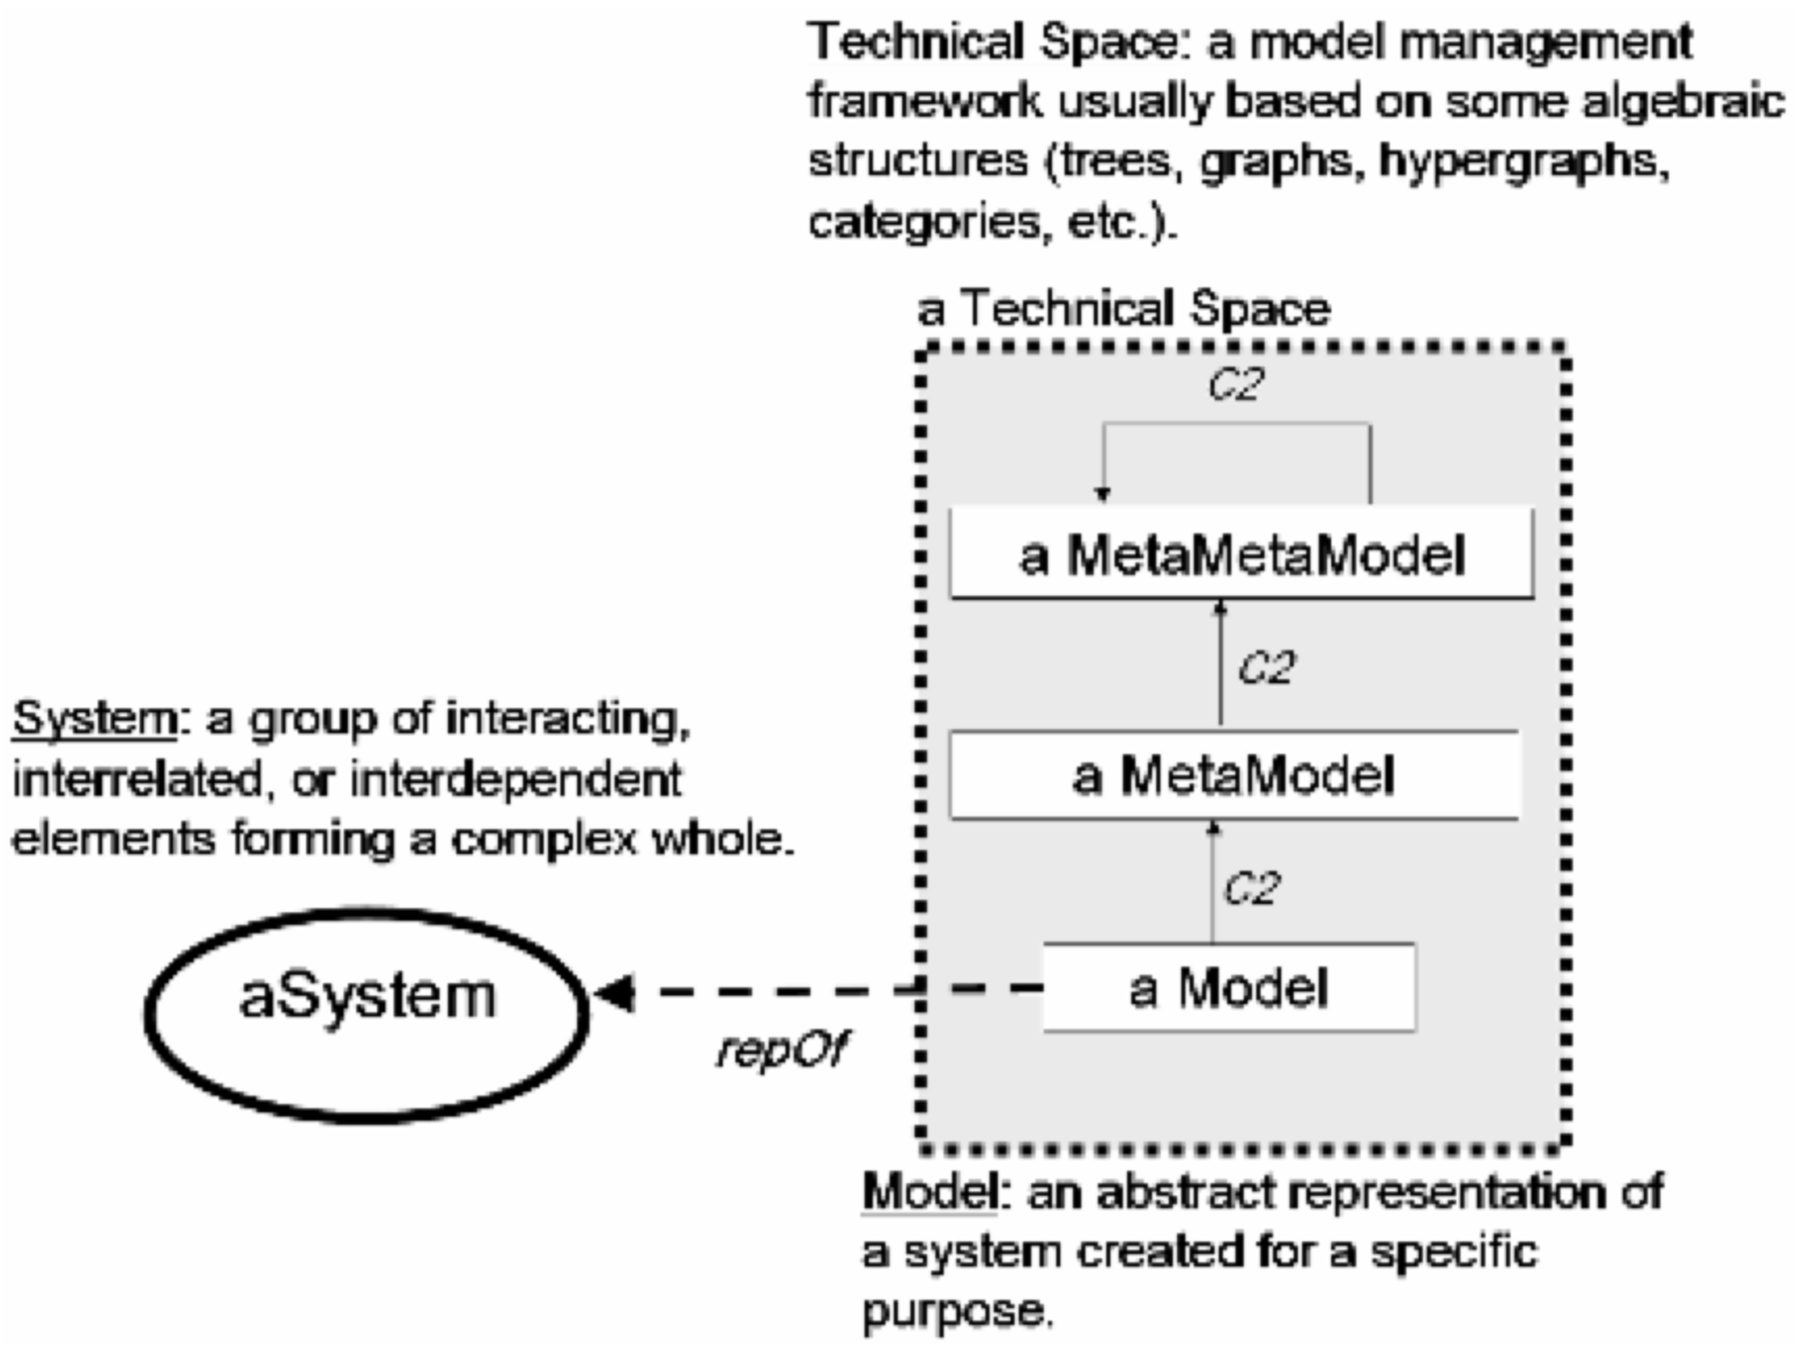
\includegraphics[width=0.6\textwidth]{bezivin2006_metamodel}
  \caption[An overview of systems, models and technical spaces]{Systems, models and technical spaces. (From \citep{Bezivin:2006gw}.)}
  \label{fig:background:metamodelling:metamodel}
\end{figure}

\noindent
\todo{How does this differ in AI context?}